% !TEX program = xelatex
% ─── Compile with XeLaTeX for Arabic + Times New Roman support ──────────────
\documentclass[12pt, a4paper, oneside]{report}

% ─── Packages ───────────────────────────────────────────────────────────────
\usepackage[top=1in, bottom=1in, left=1in, right=1in]{geometry}
\usepackage{graphicx}
\usepackage{booktabs}
\usepackage{array}
\usepackage{longtable}
\usepackage{multirow}
\usepackage{amsmath}
\usepackage{hyperref}
\usepackage{setspace}
\usepackage{titlesec}
\usepackage{fancyhdr}
\usepackage{enumitem}
\usepackage{caption}
\usepackage{float}
\usepackage{xcolor}
\usepackage{colortbl}
\usepackage{rotating}
\usepackage{needspace}
\usepackage{fontspec}
\usepackage{polyglossia}
\setmainlanguage{english}
\setotherlanguage{arabic}

\usepackage{bidi}

\newcommand{\eng}[1]{\LR{#1}}
\newcommand{\engp}[1]{\LR{(#1)}}
\setmainfont{Times New Roman}
\newfontfamily\arabicfont[Script=Arabic]{Amiri}
\usepackage{adjustbox}

\ExplSyntaxOn
\cs_if_exist:NF \tbl_save_outer_table_cols: { \cs_new:Npn \tbl_save_outer_table_cols: {} }
\ExplSyntaxOff

% ─── Line spacing ────────────────────────────────────────────────────────────
\onehalfspacing

% ─── Paragraph spacing ───────────────────────────────────────────────────────
\setlength{\parindent}{0pt}
\setlength{\parskip}{12pt}

% ─── Figure / Table numbering ────────────────────────────────────────────────
\renewcommand{\thefigure}{\thechapter-\arabic{figure}}
\renewcommand{\thetable}{\thechapter-\arabic{table}}

% ─── Caption formatting ──────────────────────────────────────────────────────
% Figure: Bold 10pt, centered, 6pt before, 24pt after
% Table:  Bold 12pt, left-aligned, 12pt before and after, title ABOVE table
\DeclareCaptionFont{bold10}{\bfseries\fontsize{10}{12}\selectfont}
\DeclareCaptionFont{bold12}{\bfseries\fontsize{12}{14}\selectfont}
\captionsetup[figure]{
  font=bold10,
  labelfont=bold10,
  justification=centering,
  skip=6pt,
  belowskip=24pt
}
\captionsetup[table]{
  font=bold12,
  labelfont=bold12,
  justification=raggedright,
  singlelinecheck=false,
  skip=12pt,
  belowskip=12pt,
  position=above
}

% ─── Chapter / Section Formatting ────────────────────────────────────────────
%
% Chapter label: Italic 14pt, letter-spacing 3.5, centered, space after 24pt
% Chapter title: Bold 16pt ALL CAPS, centered, space before 12pt, space after 36pt
%
\newcommand{\chapformat}[1]{%
  \centering
  {\fontsize{14}{17}\selectfont\itshape\addfontfeatures{LetterSpace=3.5}%
    \MakeUppercase{\chaptertitlename}\ \thechapter}\\[24pt]%
  {\fontsize{16}{19}\selectfont\bfseries\addfontfeatures{LetterSpace=0}%
    \MakeUppercase{#1}}%
}
\titleformat{\chapter}[block]
  {}{}
  {0pt}
  {\chapformat}
% space before 12pt (before entire chapter heading block), space after 36pt
\titlespacing*{\chapter}{0pt}{12pt}{36pt}

% Starred chapters (no number) — counter is saved and restored so that
% starred front-matter chapters never increment the numbered chapter counter.
\newcommand{\chapformatstar}[1]{%
  \centering
  {\fontsize{16}{19}\selectfont\bfseries\MakeUppercase{#1}}%
}
\makeatletter
\newcommand{\chapterstar}[1]{%
  \clearpage
  \phantomsection
  \edef\@saved@chapcount{\the\value{chapter}}%
  \titleformat{\chapter}[block]{}{}%
    {0pt}{\chapformatstar}%
  \@originalchapter*{#1}%
  \setcounter{chapter}{\@saved@chapcount}%
  \titleformat{\chapter}[block]{}{}%
    {0pt}{\chapformat}%
}
\let\@originalchapter\chapter
\renewcommand{\chapter}{%
  \@ifstar{\chapterstar}{\@originalchapter}%
}
\makeatother

% Heading 2: Bold 14pt ALL CAPS, left, before 18pt, after 12pt
\titleformat{\section}[hang]
  {\fontsize{14}{17}\selectfont\bfseries}
  {\thesection}{1em}{\MakeUppercase}
\titlespacing*{\section}{0pt}{18pt}{12pt}

% Heading 3: Bold 14pt Title Case, left, before 12pt, after 12pt
\titleformat{\subsection}[hang]
  {\fontsize{14}{17}\selectfont\bfseries}
  {\thesubsection}{1em}{}
\titlespacing*{\subsection}{0pt}{12pt}{12pt}

% Heading 4: Bold 13pt Title Case, left, before 12pt, after 12pt
\titleformat{\subsubsection}[hang]
  {\fontsize{13}{16}\selectfont\bfseries}
  {\thesubsubsection}{1em}{}
\titlespacing*{\subsubsection}{0pt}{12pt}{12pt}

% Heading 5: Underlined 12pt Title Case, left, before 12pt, after 12pt
\titleformat{\paragraph}[hang]
  {\fontsize{12}{14}\selectfont}
  {}{0em}{\underline}
\titlespacing*{\paragraph}{0pt}{12pt}{12pt}

% ─── Header / Footer ─────────────────────────────────────────────────────────
\pagestyle{fancy}
\setlength{\headheight}{14.5pt}
\fancyhf{}
\fancyhead[L]{\nouppercase{\leftmark}}
\fancyhead[R]{DocMind}
\fancyfoot[C]{\thepage}
\renewcommand{\headrulewidth}{0.4pt}

% ─── Hyperref ────────────────────────────────────────────────────────────────
\emergencystretch=3em
\hbadness=10000
\hfuzz=18pt

\hypersetup{
    colorlinks=true,
    linkcolor=black,
    urlcolor=blue,
    citecolor=black
}

% ─── Custom commands ─────────────────────────────────────────────────────────
\newcommand{\sigline}{\rule{5cm}{0.4pt}}

% ─── TOC orphan prevention ───────────────────────────────────────────────────
% Inject \needspace into the .toc file before every \section and \subsection
% entry so that a heading never appears alone at the bottom of a TOC page.
% This works by wrapping \section/\subsection to also write a \needspace
% command into the toc stream — it never executes in the body, only in the TOC.
\let\oldsection\section
\renewcommand{\section}{%
  \addtocontents{toc}{\protect\needspace{4\baselineskip}}%
  \oldsection
}
\let\oldsubsection\subsection
\renewcommand{\subsection}{%
  \addtocontents{toc}{\protect\needspace{3\baselineskip}}%
  \oldsubsection
}

% ─── LOF/LOT title names ─────────────────────────────────────────────────────
\renewcommand{\listfigurename}{List of Figures}
\renewcommand{\listtablename}{List of Tables}

% ─── TOC main-heading (chapter) spacing ──────────────────────────────────────
% Decrease only the vertical gap before each main (chapter) entry in the TOC.
% Implemented by redefining \l@chapter directly (rather than patching the
% class internals) so the result is identical across TeX distributions
% (e.g. local MiKTeX and Overleaf's TeX Live). This is the stock report.cls
% definition with two changes, both scoped to chapter (main-heading) entries
% only: the leading \vskip is reduced from 1.0em to 0.4em, and \parskip is
% zeroed so the document's 12pt paragraph gap is not added between entries.
\makeatletter
\renewcommand*\l@chapter[2]{%
  \ifnum \c@tocdepth >\m@ne
    \addpenalty{-\@highpenalty}%
    \vskip 0.4em \@plus\p@
    \setlength\@tempdima{1.5em}%
    \begingroup
      \parindent \z@ \parskip \z@ \rightskip \@pnumwidth
      \parfillskip -\@pnumwidth
      \leavevmode \bfseries
      \advance\leftskip\@tempdima
      \hskip -\leftskip
      #1\nobreak\hfil
      \nobreak\hb@xt@\@pnumwidth{\hss #2%
                                \kern-\p@\kern\p@}\par
      \penalty\@highpenalty
    \endgroup
  \fi}
\makeatother

% ─── List of Tables entry spacing ────────────────────────────────────────────
% Tighten the line height between List of Tables entries only. The document's
% 12pt \parskip is otherwise inserted between each entry; zeroing it here (scoped
% to \l@table) leaves the List of Figures and TOC spacing unchanged. This is the
% stock report.cls \l@table (= \l@figure) wrapped to suppress \parskip.
\makeatletter
\renewcommand*\l@table[2]{%
  \begingroup\parskip\z@
  \@dottedtocline{1}{1.5em}{2.3em}{#1}{#2}%
  \endgroup}
\makeatother

% ════════════════════════════════════════════════════════════════════════════
\begin{document}

% ─── Cover Page ─────────────────────────────────────────────────────────────
% All gaps use \vfill with weights so the content is always distributed
% across exactly one A4 page regardless of font rendering.
\begin{titlepage}
  \centering
  \thispagestyle{empty}

  % Logo
  
\includegraphics[width=3.25cm, height=3.25cm, keepaspectratio]{university_logo.png}

  \vspace{18pt}
  % University name: Bold 18pt
  {\fontsize{18}{22}\selectfont\bfseries
    Arab Academy for Science, Technology, and Maritime Transport\par}

  % Large gap after university name (template: 72pt) — use weighted fill
  \vspace{0pt plus 72pt minus 0pt}

  % College: Bold 16pt
  {\fontsize{16}{20}\selectfont\bfseries
    College of Computing and Information Technology\par}

  \vspace{18pt}

  % Department: Bold 16pt
  {\fontsize{16}{20}\selectfont\bfseries
    Department of Computer Science\par}

  % Gap after department (template: 48pt)
  \vspace{0pt plus 48pt minus 0pt}

  % Degree: Regular 14pt
  {\fontsize{14}{18}\selectfont B.Sc.\ Final Year Project\par}

  % Large gap before title (template: 72pt)
  \vspace{0pt plus 72pt minus 0pt}

  % Project title: Bold 16pt ALL CAPS
  {\fontsize{16}{20}\selectfont\bfseries DocMind\par}

  \vspace{18pt}

  % Subtitle: Bold 16pt Title Case
  {\fontsize{16}{20}\selectfont\bfseries
    AI-Powered Academic Learning Assistant\par}

  % Gap before names (template: 48pt)
  \vspace{0pt plus 48pt minus 0pt}

  % Presented By label: Regular 14pt
  {\fontsize{14}{18}\selectfont Presented By:\par}
  \vspace{6pt}

  % Student names: Italic 14pt
  {\fontsize{14}{18}\selectfont\itshape
    Abdulrhman Mohamed Gomaa \quad Ahmed Mohamed Abo El Naga \\[4pt]
    Mohamed Amgad Refat \quad Mohamed Ahmed Younes \\[4pt]
    Amr Moustafa \quad Youssef Kamal
  \par}

  \vspace{24pt}

  % Supervised By label: Regular 14pt
  {\fontsize{14}{18}\selectfont Supervised By:\par}
  \vspace{6pt}

  % Supervisor name: Italic 14pt
  {\fontsize{14}{18}\selectfont\itshape Dr.\ Ahmed Said\par}

  % Push date to footer
  \vfill

  % Month–Year: Regular 10pt
  {\fontsize{10}{12}\selectfont June 2026\par}
\end{titlepage}

% ─── Front-matter page numbering: roman numerals (i, ii, iii, …) ─────────────
\pagenumbering{roman}

% ─── Declaration ─────────────────────────────────────────────────────────────
\chapter*{Declaration}
\thispagestyle{empty}
\addcontentsline{toc}{chapter}{Declaration}

We hereby certify that this material, which we now submit for assessment on the program of study leading to the award of Bachelor of Science in Computer Science, is entirely our own work. We have exercised reasonable care to ensure that the work is original, and does not, to the best of our knowledge, breach any law of copyright, and has not been taken from the work of others save and to the extent that such work has been cited and acknowledged within the text of our work.

\vspace{1.5cm}

\noindent
\begin{tabular}{@{}p{0.48\textwidth} p{0.48\textwidth}@{}}

\textbf{Student Name:} Abdulrhman Mohamed Gomaa
& \textbf{Student Name:} Ahmed Mohamed Abo El Naga \\[6pt]

\textbf{Registration No.:} 221007510
& \textbf{Registration No.:} 221006258 \\[10pt]

\textbf{Signed:} \sigline
& \textbf{Signed:} \sigline \\[10pt]

\textbf{Date:} 29 June 2026
& \textbf{Date:} 29 June 2026 \\[30pt]

\\[20pt]

\textbf{Student Name:} Mohamed Amgad Refat
& \textbf{Student Name:} Mohamed Ahmed Younes \\[6pt]

\textbf{Registration No.:} 221006487
& \textbf{Registration No.:} 222004133 \\[10pt]

\textbf{Signed:} \sigline
& \textbf{Signed:} \sigline \\[10pt]

\textbf{Date:} 29 June 2026
& \textbf{Date:} 29 June 2026 \\[30pt]

\\[20pt]

\textbf{Student Name:} Amr Moustafa
& \textbf{Student Name:} Youssef Kamal \\[6pt]

\textbf{Registration No.:} 232004055
& \textbf{Registration No.:} 221027780 \\[10pt]

\textbf{Signed:} \sigline
& \textbf{Signed:} \sigline \\[10pt]

\textbf{Date:} 29 June 2026
& \textbf{Date:} 29 June 2026 \\

\end{tabular}

\clearpage

% ─── Abstract (English) ──────────────────────────────────────────────────────
\chapter*{Abstract}
\addcontentsline{toc}{chapter}{Abstract}

DocMind is an AI (Artificial Intelligence)-powered academic learning assistant designed to enhance the learning experience of university students by enabling reliable, document-grounded conversational interactions. The system addresses common challenges faced by students when dealing with large volumes of academic materials by allowing them to query trusted content using natural language. Unlike general-purpose AI chat systems, DocMind employs Retrieval-Augmented Generation (RAG) so that answers are grounded in an explicit corpus: instructor-uploaded materials for subject-based chat, and student-uploaded Portable Document Format (PDF) files for document-based chat.

The implemented system provides role-based access control (RBAC) for students, instructors, and administrators enforced in the Application Programming Interface (API) and web client, JSON Web Token (JWT)-based authentication with configurable token lifetime, administrator-controlled student-access gating, and validated document uploads with per-conversation limits. The backend is built on FastAPI with a PostgreSQL relational database, while semantic retrieval is powered by a pluggable vector store supporting both pgvector and Qdrant. The React-based web frontend delivers a responsive Single-Page Application (SPA) accessible across desktop and mobile browsers, complemented by a native Flutter mobile application for iOS and Android that consumes the same API. An empirical evaluation of the retrieval-augmented pipeline using the RAGAS framework over 180 questions spanning nine university subjects confirms the reliability of the document-grounded answers, achieving a faithfulness score of 0.959, context precision of 0.926, and context recall of 0.914. This document presents a comprehensive overview of the system, covering the literature review, system analysis and design, and implementation details, demonstrating the feasibility of integrating trustworthy AI-driven assistance into formal academic environments.

\clearpage

% ─── Abstract (Arabic) ───────────────────────────────────────────────────────
\chapter*{\textarabic{الملخص}}
\addcontentsline{toc}{chapter}{\textarabic{الملخص} (Arabic Abstract)}

\begin{Arabic}
\setlength{\parindent}{1.5em}
\setlength{\parskip}{6pt}

\eng{DocMind} هو مساعد تعليمي أكاديمي مدعوم بالذكاء الاصطناعي، صُمِّم لتعزيز تجربة التعلم لدى طلاب الجامعات من خلال توفير تفاعلات محادثية موثوقة ومرتكزة على المستندات. يعالج النظام التحديات الشائعة التي يواجهها الطلاب عند التعامل مع كميات كبيرة من المواد الأكاديمية، إذ يتيح لهم الاستعلام عن المحتوى الموثوق باستخدام اللغة الطبيعية.

على خلاف أنظمة الدردشة بالذكاء الاصطناعي ذات الأغراض العامة، يعتمد دوك مايند على تقنية التوليد المعزز بالاسترجاع (\eng{RAG}) بحيث ترتكز الإجابات أساساً على مجموعة محتوى محددة: المواد التي يرفعها أعضاء هيئة التدريس لمحادثات المساعد الافتراضي (الدردشة بالمادة)، والملفات التي يرفعها الطلاب أنفسهم في محادثات المستندات. يدعم النظام وضعَي تفاعل رئيسيَّين: الدردشة المرتكزة على المستندات، والدردشة المرتكزة على مواد المادة الدراسية.

يوفر النظام المُنفَّذ تحكماً في الوصول قائماً على الأدوار للطلاب والمدرسين والمسؤولين، ومصادقة مبنية على رموز \eng{JWT} مع مدة صلاحية قابلة للضبط، وبوابة للتحكم في وصول الطلاب يديرها المسؤول، فضلاً عن رفع مستندات محقَّق منها مع حدود لكل محادثة. تم بناء الواجهة الخلفية باستخدام \eng{FastAPI} مع قاعدة بيانات علائقية \eng{PostgreSQL}، فيما يعتمد الاسترجاع الدلالي على مخزن متجهات قابل للتوصيل يدعم كلاً من \eng{pgvector} و\eng{Qdrant}. تقدم الواجهة الأمامية المبنية بـ\eng{React} تطبيقاً من صفحة واحدة يعمل على أجهزة سطح المكتب والهاتف المحمول.

ويؤكد تقييم تجريبي لمسار التوليد المعزز بالاسترجاع باستخدام إطار \eng{RAGAS} على \eng{180} سؤالاً تغطي تسع مواد دراسية جامعية موثوقية الإجابات المرتكزة على المستندات، إذ حقق درجة إخلاص \engp{faithfulness} قدرها \eng{0.959}، ودقة سياق \engp{context precision} قدرها \eng{0.926}، واستدعاء سياق \engp{context recall} قدره \eng{0.914}.

يقدم هذا المستند نظرة شاملة على النظام تغطي مراجعة الأدبيات، وتحليل النظام وتصميمه، وتفاصيل التنفيذ، مما يعكس التطبيق الفعلي للمستودع ويُثبت جدوى دمج المساعدة الموثوقة المدعومة بالذكاء الاصطناعي في البيئات الأكاديمية الرسمية.

\end{Arabic}

\clearpage

% ─── Dedication ──────────────────────────────────────────────────────────────
\chapter*{Dedication}
\addcontentsline{toc}{chapter}{Dedication}
\thispagestyle{fancy}

\vspace*{\fill}
\begin{center}
  \textit{To our families, whose patience and support made this journey possible.}\\[6pt]
  \textit{To our supervisor, Dr.\ Ahmed Said, for his invaluable guidance.}\\[6pt]
  \textit{And to every student who deserves a smarter, more accessible way to learn.}
\end{center}
\vspace*{\fill}

\clearpage

% ─── Acknowledgments ─────────────────────────────────────────────────────────
\chapter*{Acknowledgments}
\addcontentsline{toc}{chapter}{Acknowledgments}

We would like to express our sincere gratitude to Dr.\ Ahmed Said for his continuous guidance, insightful feedback, and unwavering support throughout the development of this project. His expertise and encouragement were instrumental in shaping both the academic and technical aspects of DocMind.

We also extend our thanks to the faculty and staff of the College of Computing and Information Technology at the Arab Academy for Science, Technology, and Maritime Transport, for providing an environment conducive to research and innovation.

Special appreciation goes to our families and friends for their patience, encouragement, and moral support during the many hours invested in this project.

Finally, we acknowledge the open-source communities behind FastAPI, React, PostgreSQL, LangChain, pgvector, and Qdrant, whose contributions to the software ecosystem made the technical realization of DocMind possible.

\clearpage

% ─── Table of Contents ───────────────────────────────────────────────────────
% Tighten line height across all TOC entries by zeroing the document's 12pt
% \parskip for the duration of the TOC (section/subsection entries otherwise
% inherit it). Scoped in a group so the body spacing is unchanged afterwards.
\begingroup
\setlength{\parskip}{0pt}
\tableofcontents
\endgroup
\clearpage

% ─── List of Tables ──────────────────────────────────────────────────────────
\clearpage
\listoftables
\addcontentsline{toc}{chapter}{List of Tables}
\clearpage

% ─── List of Figures ─────────────────────────────────────────────────────────
% Zero \parskip and neutralize the \addvspace{10pt} LaTeX inserts between
% figures of different chapters, so all entries are tightly spaced. Scoped in
% a group so body spacing is unchanged afterwards.
\clearpage
\begingroup
\setlength{\parskip}{0pt}
\let\oldaddvspace\addvspace
\renewcommand{\addvspace}[1]{}
\listoffigures
\let\addvspace\oldaddvspace
\endgroup
\addcontentsline{toc}{chapter}{List of Figures}
\clearpage

% ─── List of Acronyms ────────────────────────────────────────────────────────
\chapter*{List of Acronyms / Abbreviations}
\addcontentsline{toc}{chapter}{List of Acronyms / Abbreviations}

\begin{tabular}{>{\bfseries}p{3.5cm} p{11cm}}
\toprule
Acronym & Definition \\
\midrule
AI    & Artificial Intelligence \\
API   & Application Programming Interface \\
CLI   & Command-Line Interface \\
CRUD  & Create, Read, Update, Delete \\
CSS   & Cascading Style Sheets \\
DB    & Database \\
ERD   & Entity-Relationship Diagram \\
GDPR  & General Data Protection Regulation \\
HTTP  & Hypertext Transfer Protocol \\
HTTPS & Hypertext Transfer Protocol Secure \\
ICL   & In-Context Learning \\
JSON  & JavaScript Object Notation \\
JWT   & JSON Web Token \\
LLM   & Large Language Model \\
LMS   & Learning Management System \\
NLP   & Natural Language Processing \\
PDF   & Portable Document Format \\
PEFT  & Parameter-Efficient Fine-Tuning \\
PostgreSQL & Post Ingres Structured Query Language \\
RAG   & Retrieval-Augmented Generation \\
RBAC  & Role-Based Access Control \\
REST  & Representational State Transfer \\
SPA   & Single-Page Application \\
SQL   & Structured Query Language \\
SRS   & Software Requirements Specification \\
SSO   & Single Sign-On \\
TLS   & Transport Layer Security \\
UI    & User Interface \\
UML   & Unified Modeling Language \\
URL   & Uniform Resource Locator \\
UX    & User Experience \\
\bottomrule
\end{tabular}

\clearpage

% ════════════════════════════════════════════════════════════════════════════
%  CHAPTER 1 — INTRODUCTION
% ════════════════════════════════════════════════════════════════════════════
% ─── Main-matter page numbering: arabic numerals (1, 2, 3, …) ────────────────
\pagenumbering{arabic}
\chapter{Introduction}

\section{Background}

The rapid advancement of information technology has significantly transformed modern educational environments. Universities and academic institutions increasingly rely on digital platforms to distribute learning materials, manage coursework, and facilitate communication between instructors and students. Lecture notes, presentations, assignments, and supplementary references are now commonly delivered through online Learning Management Systems (LMS), shared repositories, and institutional portals.

While this digital transformation has improved accessibility and flexibility, it has also introduced new challenges. Students are often required to process large volumes of academic material within limited timeframes. Navigating these materials efficiently, identifying relevant information, and fully understanding complex concepts has become increasingly difficult. Traditional learning methods, such as manual document reading or keyword-based searching, are often insufficient to support effective comprehension in such data-heavy environments.

At the same time, recent advancements in Artificial Intelligence (AI), particularly in Natural Language Processing (NLP), have enabled the development of conversational systems capable of interacting with users in human-like ways. These systems have demonstrated potential in education by providing personalized assistance, answering questions, and supporting self-directed learning in [6]. However, the integration of such technologies into formal academic environments requires careful consideration to ensure accuracy, reliability, and alignment with educational objectives.

\newpage

\section{Problem Statement}

Despite the availability of extensive academic resources, students frequently encounter difficulties in extracting meaningful knowledge from them. Large documents such as lecture slides and textbooks often contain dense information, making it challenging for students to locate specific answers or clarify particular concepts efficiently. As a result, students may resort to external sources that are not aligned with course content, or may receive incomplete or misleading explanations.

Generic AI chat systems have gained popularity as tools for answering questions and providing explanations. However, these systems are typically trained on broad datasets and are not restricted to verified academic sources. Consequently, they may generate responses that are factually incorrect, inconsistent with course materials, or entirely fabricated, a phenomenon Known as AI hallucination in [7]. Such behavior poses significant risks in academic contexts, where accuracy and reliability are essential.

Furthermore, instructors often face repetitive questions from students regarding course materials, which can increase workload and reduce time available for higher-level academic engagement. There is a clear need for a system that can provide consistent, accurate, and course-aligned assistance while reducing reliance on unreliable external tools.

\section{Motivation}

The motivation behind the DocMind project arises from the need to bridge the gap between traditional academic content and intelligent learning assistance. The project aims to leverage modern AI techniques while addressing the limitations and risks associated with unrestricted language models in education.

DocMind is motivated by the concept of grounded intelligence, where AI-generated responses are explicitly tied to trusted and verified sources. By restricting the system's knowledge base to instructor-approved documents and uploaded academic materials, DocMind seeks to ensure that all responses remain aligned with course objectives and institutional standards.

Another key motivation is to support self-directed learning. Students often learn at different paces and require varying levels of explanation. An interactive academic assistant allows students to ask questions freely, revisit concepts multiple times, and explore topics in greater depth without time constraints. This flexibility promotes independent learning while maintaining academic integrity.

\newpage

\section{Objectives}

The primary objective of the DocMind project is to design and implement an AI-powered academic learning assistant that provides accurate, reliable, and context-aware support for university students. To achieve this goal, the project defines several specific objectives:

\begin{itemize}
  \item To enable natural language interaction with academic documents and course materials.
  \item To ensure that all generated responses are grounded in verified and instructor-approved sources.
  \item To reduce the occurrence of AI hallucinations and misinformation in educational contexts.
  \item To support instructors by minimizing repetitive clarification requests.
  \item To provide a scalable and maintainable system architecture suitable for institutional deployment.
  \item To promote ethical and responsible use of artificial intelligence in education.
\end{itemize}

These objectives guide both the functional requirements and the design decisions of the system, ensuring alignment between user needs and technical implementation.

\section{Scope}

The scope of the DocMind project includes the design and development of an academic assistant integrated within a university environment. The system supports two primary modes of interaction: document-based chat, where students interact with uploaded documents, and subject-based chat, which relies on instructor-managed course materials.

The project focuses on system architecture, user interaction design, database design, and AI integration using Retrieval-Augmented Generation (RAG) techniques [5]. The system is designed to operate within defined constraints, such as authenticated session expiry via JSON Web Token (JWT), per-role authorization, per-conversation upload limits and file-type validation, and administrator policies including optional disabling of student access, to ensure relevance and reliability.

The project does not aim to replace instructors, tutors, or formal assessment methods. Instead, DocMind functions as a supplementary learning tool that enhances understanding and supports academic engagement. Features such as grading automation or autonomous decision-making are explicitly outside the scope of this project.

\newpage

\section{Organization of the Document}

This document is organized into five chapters to provide a comprehensive and structured presentation of the DocMind system.

\begin{enumerate}
  \item \textbf{Chapter 1 (Introduction)} introduces the project background, problem statement, motivation, objectives, and overall scope of the system.
  \item \textbf{Chapter 2 (Literature Review)} presents a detailed review of relevant research papers, market analysis, related projects, and similar existing systems, highlighting existing approaches and their implications for the proposed solution.
  \item \textbf{Chapter 3 (Proposed Work --- System Analysis and Design)} describes the overall behavior of the DocMind system, including functional and nonfunctional requirements, system architecture, AI pipeline design, database design, and Unified Modeling Language (UML) diagrams.
  \item \textbf{Chapter 4 (Implementation and Testing)} documents the repository-backed implementation, interface walkthroughs for all user roles, prototype evaluation, and testing considerations.
  \item \textbf{Chapter 5 (Conclusions and Future Work)} presents conclusions validating the project and outlines planned enhancements and directions for future development.
\end{enumerate}

% ════════════════════════════════════════════════════════════════════════════
%  CHAPTER 2 — LITERATURE REVIEW
% ════════════════════════════════════════════════════════════════════════════
\chapter{Literature Review}

This chapter presents a review of relevant academic research related to artificial intelligence in education, conversational learning systems, and document-grounded AI models. It also provides a market analysis and survey of similar systems currently available. The reviewed papers provide foundational insights that inform the design and implementation of the DocMind system. Rather than merely summarizing prior work, this chapter discusses the implications of each study for the DocMind approach, identifying strengths, limitations, and design decisions that arise from the literature.

\section{Research Papers}

This section reviews four research papers that examine fine-tuning and Retrieval-Augmented Generation (RAG), highlighting their performance, limitations, and suitability for the DocMind application.

% ─────────────────────────────────────────────────────────────────────────────
\subsection{Paper 1: Comparing Retrieval-Augmentation and Parameter Efficient Fine-Tuning for Privacy-Preserving Personalization of Large Language Models}

\textbf{Authors}: Hamed Zamani, Alireza Salemi [1]\\
\textbf{Published at}: 26 Jun 2025, University of Massachusetts


\subsubsection{Overview}

This paper compares retrieval-augmented generation (RAG) and parameter-efficient fine-tuning (PEFT) for privacy-preserving personalization of large language models (LLMs). Results show that RAG outperforms PEFT when data is limited, while PEFT improves with larger profiles. Combining them achieves the best personalization performance without violating privacy.

\subsubsection{The Dataset}

LaMP datasets with different personalized fields:
\begin{itemize}[noitemsep]
  \item LaMP-1 (Citation)
  \item LaMP-2 (Movie Tagging)
  \item LaMP-3 (Product Rating)
  \item LaMP-7 (Tweet Paraphrasing)
\end{itemize}


\subsubsection{Methodology}

\paragraph{PEFT-RAG for Personalizing LLMs by Two Approaches:}

\begin{enumerate}
  \item \textbf{Personalizing the Input Prompt}: This approach modifies the input prompt given to the model to encourage it to generate responses that are more tailored to the specific user's needs.
  \item \textbf{Changing the Model Parameters}: This approach involves training the LLM with user-specific data, allowing the model to learn the user's preferences.
\end{enumerate}

This approach combines Parameter-Efficient Fine-Tuning (PEFT) and Retrieval-Augmented Generation (RAG) to enhance the personalization of large language models by:

\begin{itemize}[noitemsep]
    \item \textbf{PEFT:} Fine-tunes a small set of additional parameters, reducing computational and memory overhead.

    \item \textbf{RAG:} Mitigates the limitations of PEFT by dynamically retrieving user-specific information during inference.
\end{itemize}
\newpage
\subsubsection{Comparison of Different Techniques}

The following table compares the methods described: RAG, PEFT, and PEFT-RAG. As shown in Table~\ref{tab:lamp_comparison}, the combination of both techniques consistently yields the highest personalization scores across the LaMP benchmark tasks.

\begin{table}[H]
\centering
\caption{Comparison of Personalization Techniques Across LaMP Datasets}
\label{tab:lamp_comparison}
\scriptsize
\setlength{\tabcolsep}{3pt}
\renewcommand{\arraystretch}{1.2}
\begin{adjustbox}{max width=\textwidth}
\begin{tabular}{>{\raggedright\arraybackslash}p{3.2cm} l c cccc cccc cccc}
\toprule
\multirow{2}{=}{\textbf{Dataset}} & \multirow{2}{*}{\textbf{Metric}}
  & \textbf{No}
  & \multicolumn{4}{c}{\textbf{PEFT Personalization}}
  & \multicolumn{4}{c}{\textbf{RAG Personalization}}
  & \multicolumn{4}{c}{\textbf{PEFT-RAG Personalization}} \\
\cmidrule(lr){4-7} \cmidrule(lr){8-11} \cmidrule(lr){12-15}
 & & \textbf{Pers.}
  & $r{=}8$ & $r{=}16$ & $r{=}32$ & $r{=}64$
  & BM25 & Recency & Contriever & RSPG
  & $r{=}8$ & $r{=}16$ & $r{=}32$ & $r{=}64$ \\
\midrule
LaMP-1: Personalized Citation Identification & Accuracy $\uparrow$
  & 0.502 & 0.502 & 0.502 & 0.504 & 0.506
  & 0.626 & 0.622 & 0.636 & \textbf{0.672}
  & 0.670 & 0.668 & 0.671 & 0.671 \\
\midrule
\multirow{2}{=}{LaMP-2: Personalized Movie Tagging} & Accuracy $\uparrow$
  & 0.359 & 0.360 & 0.360 & 0.360 & 0.359
  & 0.387 & 0.377 & 0.396 & 0.430
  & 0.430 & \textbf{0.431} & 0.430 & 0.430 \\
 & F1 $\uparrow$
  & 0.276 & 0.278 & 0.278 & 0.278 & 0.277
  & 0.306 & 0.295 & 0.304 & 0.339
  & 0.341 & \textbf{0.342} & 0.341 & 0.341 \\
\midrule
\multirow{2}{=}{LaMP-3: Personalized Product Rating} & MAE $\downarrow$
  & 0.308 & 0.308 & 0.307 & 0.306 & 0.301
  & 0.298 & 0.296 & 0.299 & 0.264
  & 0.264 & 0.265 & 0.264 & \textbf{0.259} \\
 & RMSE $\downarrow$
  & 0.611 & 0.607 & 0.607 & 0.602 & 0.600
  & 0.611 & 0.605 & 0.616 & 0.568
  & 0.568 & 0.570 & 0.564 & \textbf{0.562} \\
\midrule
\multirow{2}{=}{LaMP-4: Personalized News Headline Generation} & ROUGE-1 $\uparrow$
  & 0.176 & 0.178 & 0.177 & 0.178 & 0.178
  & 0.186 & 0.189 & 0.183 & 0.203
  & 0.203 & \textbf{0.204} & \textbf{0.204} & 0.203 \\
 & ROUGE-L $\uparrow$
  & 0.160 & 0.162 & 0.162 & 0.163 & 0.163
  & 0.171 & 0.173 & 0.169 & 0.186
  & 0.186 & 0.186 & \textbf{0.187} & 0.186 \\
\midrule
\multirow{2}{=}{LaMP-5: Personalized Scholarly Title Generation} & ROUGE-1 $\uparrow$
  & 0.478 & 0.478 & 0.478 & 0.477 & 0.478
  & 0.477 & 0.475 & \textbf{0.483} & 0.480
  & 0.481 & 0.480 & 0.480 & 0.479 \\
 & ROUGE-L $\uparrow$
  & 0.428 & 0.429 & 0.429 & 0.428 & 0.428
  & 0.427 & 0.426 & \textbf{0.433} & 0.429
  & 0.431 & 0.431 & 0.431 & 0.431 \\
\midrule
\multirow{2}{=}{LaMP-6: Personalized Email Subject Generation} & ROUGE-1 $\uparrow$
  & 0.335 & 0.342 & 0.342 & 0.341 & 0.343
  & 0.412 & 0.403 & 0.401 & 0.433
  & 0.436 & 0.436 & 0.436 & \textbf{0.437} \\
 & ROUGE-L $\uparrow$
  & 0.319 & 0.325 & 0.326 & 0.325 & 0.326
  & 0.398 & 0.389 & 0.386 & 0.418
  & \textbf{0.422} & \textbf{0.422} & \textbf{0.422} & 0.421 \\
\midrule
\multirow{2}{=}{LaMP-7: Personalized Tweet Paraphrasing} & ROUGE-1 $\uparrow$
  & 0.449 & 0.449 & 0.449 & 0.449 & 0.449
  & 0.446 & 0.444 & 0.440 & \textbf{0.461}
  & 0.460 & 0.460 & 0.460 & 0.460 \\
 & ROUGE-L $\uparrow$
  & 0.396 & 0.397 & 0.397 & 0.396 & 0.396
  & 0.394 & 0.393 & 0.390 & \textbf{0.409}
  & \textbf{0.409} & \textbf{0.409} & 0.408 & \textbf{0.409} \\
\bottomrule
\end{tabular}
\end{adjustbox}
\end{table}

\subsubsection{Main Findings}

The combination of PEFT-trained personalized LLMs and RAG retrieval models resulted in:

\begin{enumerate}[label=\alph*-]
  \item 15.98\% improvement over the non-personalized LLM.
  \item Outperforming standard RAG in 4 out of 7 tasks, showing that PEFT enhances personalization by fine-tuning the model alongside real-time retrieval.
\end{enumerate}

\subsubsection{Drawbacks}

\begin{enumerate}
  \item RAG suffers from retrieval latency, particularly as the profile size increases.
  \item PEFT is constrained by adapter loading overhead, which can impact real-time applications requiring frequent updates.
\end{enumerate}

\subsubsection{Implications for DocMind}

The findings from this paper reinforce the decision to use RAG as the primary retrieval strategy in DocMind. Given that DocMind operates on institutional document corpora with no per-student parametric fine-tuning, the RAG-only approach remains practical, cost-effective, and privacy-preserving. Fine-tuning could be explored in future work once sufficient interaction data is available.

% ─────────────────────────────────────────────────────────────────────────────
\subsection{Paper 2: A Comparison of Independent and Joint Fine-Tuning Strategies for Retrieval-Augmented Generation}

\textbf{Authors}: Neal Lawton, Alfy Samuel, Anoop Kumar, Daben Liu [2]\\
\textbf{Published at}: 17 Oct 2025, Cornell University

\subsubsection{Overview}

This paper compares independent, joint, and two-phase fine-tuning strategies for retrieval-augmented generation (RAG) systems. Experiments show that all strategies achieve similar answer quality improvements, but differ greatly in computational cost. The optimal strategy depends on whether context labels are available and whether extensive learning-rate tuning is required.

\subsubsection{The Dataset}

\begin{enumerate}
  \item \textbf{HotPotQA} dataset including 113k Questions and Answers with distractors to make the reasoning harder and test the fine-tuning performance (general).
  \item \textbf{PopQA} dataset: a smaller dataset containing 30k question-and-answer pairs including distractors (more specific).
\end{enumerate}
\newpage
\subsubsection{Methodology}

The paper evaluates five techniques for applying RAG:

\begin{enumerate}
  \item No fine-tuning.
  \item Fine-tuning the embedded vector in the RAG pipeline.
  \item Fine-tuning the LLM Generator (highly recommended).
  \item Fine-tuning both the RAG pipeline and the LLM Generator (joint fine-tuning).
  \item Two-phase fine-tuning (fine-tuning the embedded vector alone, followed by fine-tuning the generator alone, then balancing between them).
\end{enumerate}

\paragraph{Diagram of Different Techniques:}\mbox{}\\


\begin{figure}[H]
  \centering
  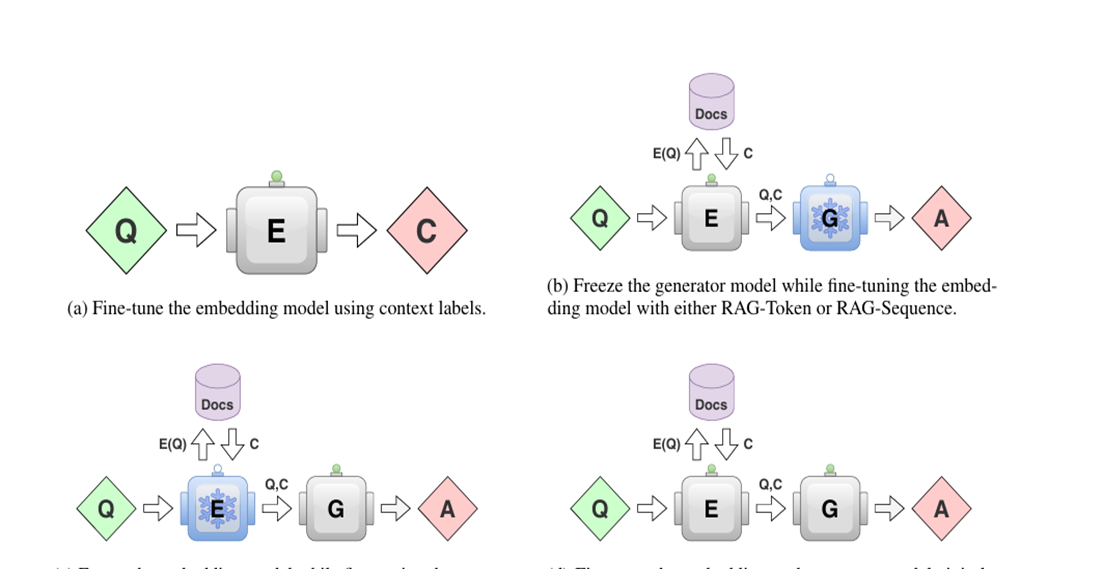
\includegraphics[width=0.85\textwidth]{rag_techniques_diagram.png}
  \caption{Different fine-tuning techniques for RAG pipelines: (a) fine-tune embedding model using context labels; (b) freeze generator while fine-tuning the embedding model; (c) fine-tune embedding model jointly; (d) two-phase fine-tuning.}
  \label{fig:rag_techniques}
\end{figure}

\newpage

\subsubsection{Models Evaluation}

Table~\ref{tab:hotpot_eval} and Figure~\ref{fig:models_eval} present the evaluation results for each fine-tuning strategy across both datasets.

\begin{figure}[H]
  \centering
  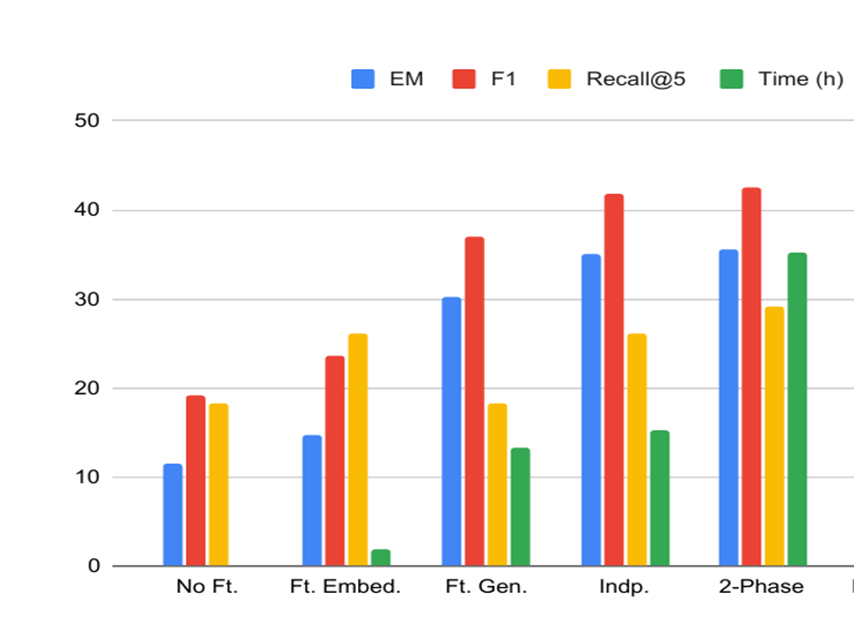
\includegraphics[width=0.85\textwidth]{models_evaluation_chart.png}
  \caption{Model evaluation results comparing Exact Match (EM), F1, Recall@5, and Time (h) across fine-tuning strategies.}
  \label{fig:models_eval}
\end{figure}

\begin{table}[H]
\centering
\caption{Evaluation Results on HotPotQA and PopQA}
\label{tab:hotpot_eval}
\begin{tabular}{lcccccccc}
\toprule
\multirow{2}{*}{Method} & \multicolumn{4}{c}{HotPotQA} & \multicolumn{4}{c}{PopQA} \\
\cmidrule(lr){2-5}\cmidrule(lr){6-9}
 & Exact Match & F1 & Recall@5 & Time (h) & Exact Match & F1 & Recall@5 & Time (h) \\
\midrule
No Ft.      & 10.3 & 19.8 & 19.1 &  0.0 & 12.6 & 18.6 & 17.4 & 0   \\
Ft. Embed.  & 11.1 & 20.8 & 21.4 &  3.5 & 18.2 & 26.6 & 30.8 & 0.4 \\
Ft. Gen.    & 28.4 & 39.4 & 19.1 & 23.8 & 32.1 & 34.7 & 17.4 & 2.9 \\
Indp.       & 29.3 & 40.2 & 21.4 & 27.4 & 40.6 & 43.2 & 30.8 & 3.2 \\
2-Phase     & 30.0 & 41.3 & 25.1 & 61.0 & 41.0 & 43.7 & 33.3 & 9.4 \\
\bottomrule
\end{tabular}
\end{table}

\subsubsection{Conclusion}

Fine-tuning the generator only is the most realistic option for DocMind as it is more affordable to implement than joint fine-tuning and two-phase fine-tuning. It also yields acceptable results in large datasets, making it suitable for this use case. Finally, it is comparatively affordable compared to more complex fine-tuning techniques.

\subsubsection{Implications for DocMind}

This paper confirms that generator fine-tuning offers a practical middle ground between raw RAG and computationally expensive joint strategies. For DocMind, where inference budget and operational simplicity are priorities, generator-only fine-tuning represents a viable future enhancement that does not require restructuring the retrieval pipeline.

% ─────────────────────────────────────────────────────────────────────────────
\newpage
\subsection{Paper 3: Fine-Tuning or Fine-Failing? Debunking Performance Myths in Large Language Models}

\textbf{Authors}: Scott Barnett, Zac Brannelly, Stefanus, Sheng Wong [3]\\
\textbf{Published at}: 17 Jun 2025, Deakin University

\subsubsection{Overview}

This paper investigates whether fine-tuning large language models improves performance when used inside RAG pipelines. Experiments across multiple datasets show that fine-tuned models often perform worse than baseline models in both accuracy and completeness. The findings challenge the assumption that fine-tuning always helps, emphasizing the need for careful validation in domain-specific RAG settings.

\subsubsection{The Dataset}

The researchers tested their approach on three publicly available question-and-answer datasets, each from a different domain:

\paragraph{BioASQ:}
\begin{itemize}[noitemsep]
  \item Biomedical question-and-answer dataset
  \item 15,000 documents
  \item 1,000 expert-created question-and-answer pairs for fine-tuning
\end{itemize}

\paragraph{Natural Questions (NQ):}
A large-scale open-ended question-and-answer dataset containing real Google search queries with answers linked to Wikipedia pages.

\paragraph{QASPER:}
\begin{itemize}[noitemsep]
  \item Dataset from NLP research papers
  \item 5,049 questions from 1,585 scientific papers
\end{itemize}

\subsubsection{Methodology}

\begin{enumerate}
  \item \textbf{Models}: LLaMA-2, Mistral, and GPT-4
  \item \textbf{Fine-Tuning}: Fine-tuned LLaMA-2 and Mistral on 200 samples, 500 samples, and 1,000 samples using LoRA / QLoRA for efficient fine-tuning. Hardware: A100/H100 GPUs.
  \item \textbf{RAG}: For each question, the top 5 similar chunks were retrieved from the dataset, concatenated into one context block, and passed with the question to the model.
\end{enumerate}

\subsubsection{Comparison}

Figure~\ref{fig:llama2_accuracy} and Figure~\ref{fig:mixtral_accuracy} show the accuracy of fine-tuned models across all three datasets, demonstrating that fine-tuning consistently failed to improve results over the baseline.

\begin{figure}[H]
  \centering
  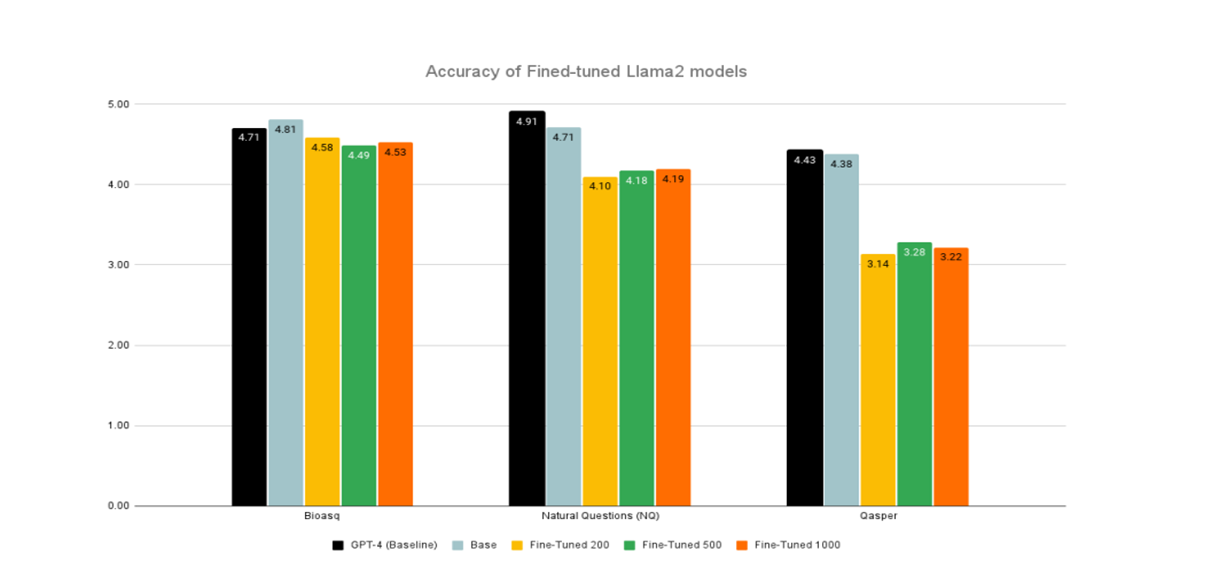
\includegraphics[width=0.85\textwidth]{finetuned_llama2_chart.png}
  \caption{Accuracy of fine-tuned LLaMA-2 models across BioASQ, Natural Questions (NQ), and QASPER datasets.}
  \label{fig:llama2_accuracy}
\end{figure}

\begin{figure}[H]
  \centering
  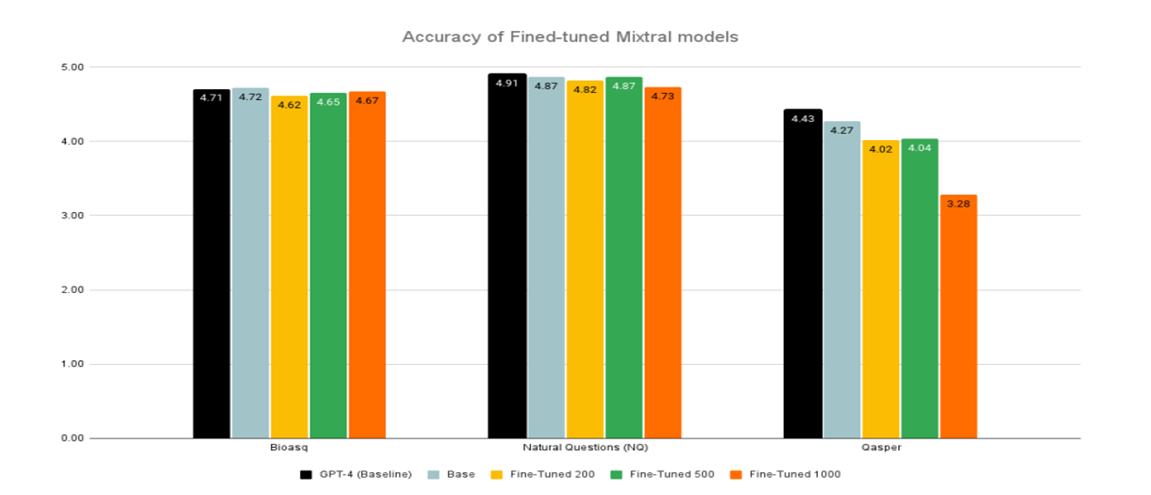
\includegraphics[width=0.85\textwidth]{finetuned_mixtral_chart.png}
  \caption{Accuracy of fine-tuned Mistral models across BioASQ, Natural Questions (NQ), and QASPER datasets.}
  \label{fig:mixtral_accuracy}
\end{figure}

\begin{enumerate}
  \item Fine-tuning made the models perform worse.
  \item The baseline (original) LLMs gave more accurate and complete answers than the fine-tuned versions.
  \item Increasing dataset size from 200 to 500 to 1000 samples did not improve results, and in some cases made them worse.
  \item Limitation of hardware resources negatively affects the fine-tuning process.
\end{enumerate}

\subsubsection{Implications for DocMind}

The results in [3] directly validate the decision to avoid fine-tuning in the DocMind prototype. In specialized, document-grounded educational settings, the cost and risk of fine-tuning outweigh potential gains. Retrieval quality and prompt engineering are more reliable levers for improving answer quality, and these are the strategies adopted in the DocMind pipeline.

% ─────────────────────────────────────────────────────────────────────────────
\newpage
\subsection{Paper 4: Enhancing Retrieval-Augmented Generation: A Study of Best Practices}

\textbf{Authors}: Siran Li, Linus Stenzel, Carsten Eickhoff, Seyed Ali [4]\\
\textbf{Published at}: 13 Jan 2025, University of T\"{u}bingen

\subsubsection{Overview}

This paper systematically studies best practices for designing high-performance Retrieval-Augmented Generation (RAG) systems through extensive ablation experiments. Results show that Contrastive In-Context Learning (ICL) RAG and Focus Mode RAG consistently outperform other variants, especially on knowledge-intensive tasks such as the Massive Multitask Language Understanding (MMLU) benchmark. The study concludes that retrieval quality, prompt design, and targeted context selection matter more than larger knowledge bases or aggressive retrieval strategies.

\subsubsection{The Dataset}

\paragraph{TruthfulQA:}
\begin{itemize}[noitemsep]
  \item 817 questions across 38 categories
  \item Tests commonsense knowledge and truthfulness
  \item Includes correct and incorrect answers for evaluation
\end{itemize}

\paragraph{MMLU (Massive Multitask Language Understanding):}
\begin{itemize}[noitemsep]
  \item Educational and professional domains, 57 subjects
  \item Multiple-choice questions (1824 samples used for evaluation)
  \item Requires precise and specialized knowledge
\end{itemize}

\newpage
\subsubsection{Methodology}

\paragraph{Query Expansion Module:}
\begin{itemize}[noitemsep]
  \item Uses Flan-T5 to expand queries for more relevant retrieval.
\end{itemize}

\paragraph{Retrieval Module:}
\begin{itemize}[noitemsep]
  \item Uses FAISS [14] with Sentence Transformers for semantic search.
  \item Documents split into chunks; Focus Mode retrieves only the most relevant sentences.
\end{itemize}

\paragraph{Text Generation Model (LLM):}
\begin{itemize}[noitemsep]
  \item Mistral models (7B and 45B) generate responses based on retrieved context.
\end{itemize}

\subsubsection{Comparison}

Table~\ref{tab:ablation_comparison} summarizes the ablation study results across TruthfulQA and MMLU, comparing all RAG configurations evaluated in [4].

\begin{table}[H]
\centering
\caption{Ablation Study Results on TruthfulQA and MMLU}
\label{tab:ablation_comparison}
\footnotesize
\setlength{\tabcolsep}{3pt}
\begin{tabular}{llccccccccccc}
\toprule
 & & \multicolumn{5}{c}{\textbf{TruthfulQA}} & \multicolumn{5}{c}{\textbf{MMLU}} \\
\cmidrule(lr){3-7}\cmidrule(lr){8-12}
 & & R1 & R2 & RL & ECS & Mauve & R1 & R2 & RL & ECS & Mauve \\
\midrule
\multirow{2}{*}{LLM Size}
  & Instruct7B  & 26.81 & 13.26 & 23.86 & 56.44 & 72.92 & 10.42 & 1.90 & 8.91 & 29.41 & 40.51 \\
  & Instruct45B & 29.07 & 14.95 & 25.64 & 58.63 & 81.62 & 11.06 & 2.05 & 9.37 & 30.82 & 38.24 \\
\midrule
\multirow{5}{*}{\shortstack[l]{Prompt\\Design}}
  & HelpV1   & 26.81 & 13.26 & 23.86 & 56.44 & 72.92 & 10.42 & 1.90 & 8.91 & 29.41 & 40.51 \\
  & HelpV2   & 27.00 & 13.88 & 23.93 & 57.33 & 75.38 & 10.21 & 1.80 & 8.77 & 29.45 & 36.20 \\
  & HelpV3   & 26.30 & 13.01 & 23.16 & 56.54 & 79.20 & 10.40 & 1.97 & 9.00 & 29.39 & 34.50 \\
  & AdversV1 & 10.06 & 1.60  & 8.60  & 19.78 & 2.55  & 6.58  & 0.72 & 5.75 & 14.04 & 4.05  \\
  & AdversV2 & 8.39  & 2.14  & 7.48  & 16.30 & 0.93  & 4.24  & 0.54 & 3.84 & 12.33 & 0.76  \\
\midrule
\multirow{4}{*}{\shortstack[l]{Doc\\Size}}
  & 2DocS  & 27.41 & 13.71 & 24.27 & 57.52 & 78.53 & 10.43 & 1.92 & 8.88 & 29.44 & 38.22 \\
  & 2DocM  & 26.81 & 13.26 & 23.86 & 56.44 & 72.92 & 10.42 & 1.90 & 8.91 & 29.41 & 40.51 \\
  & 2DocL  & 26.96 & 13.78 & 23.92 & 57.00 & 82.02 & 10.41 & 1.88 & 8.88 & 29.52 & 36.21 \\
  & 2DocXL & 27.60 & 13.98 & 24.46 & 57.66 & 76.44 & 10.54 & 1.95 & 9.00 & 29.67 & 39.35 \\
\midrule
\multirow{4}{*}{\shortstack[l]{Contrastive\\ICL}}
  & Baseline & 26.81 & 13.26 & 23.86 & 56.44 & 72.92 & 10.42 &  1.90 &  8.91 & 29.41 & 40.51 \\
  & ICL1Doc  & 29.25 & 15.82 & 26.14 & 56.93 & 67.41 & 20.47 & 11.40 & 18.96 & 41.85 & 33.94 \\
  & ICL2Doc  & 28.62 & 16.05 & 25.68 & 56.07 & 66.87 & 23.23 & 14.66 & 22.02 & 43.09 & 34.20 \\
  & ICL1Doc+ & \textbf{30.62} & \textbf{17.45} & \textbf{27.79} & \textbf{58.96} & \textbf{73.86} & 25.09 & 15.87 & 23.87 & \textbf{47.12} & \textbf{43.50} \\
  & ICL2Doc+ & 30.24 & 17.77 & 27.51 & 57.55 & 67.51 & \textbf{26.01} & \textbf{17.46} & \textbf{24.90} & 47.04 & 37.24 \\
\midrule
\multirow{6}{*}{\shortstack[l]{Focus\\Mode}}
  & Baseline   & 26.81 & 13.26 & 23.86 & 56.44 & 72.92 & 10.42 & 1.90 & 8.91 & 29.41 & 40.51 \\
  & 2Doc1S     & 26.11 & 12.37 & 23.05 & 55.65 & 73.02 & 10.77 & \textbf{2.13} & \textbf{9.25} & 29.90 & 41.00 \\
  & 20Doc20S   & 28.20 & 14.48 & 24.90 & 58.30 & 74.02 & 10.64 & 1.99 & 9.11 & 30.03 & 39.18 \\
  & 40Doc40S   & 28.32 & 14.54 & 24.99 & \textbf{58.36} & \textbf{77.95} & 10.78 & 2.02 & 9.20 & 30.01 & 36.20 \\
  & 80Doc80S   & \textbf{28.85} & \textbf{15.01} & \textbf{25.51} & 58.33 & 74.15 & 10.69 & 2.04 & 9.15 & 29.97 & 38.09 \\
  & 120Doc120S & 28.36 & 14.80 & 25.09 & 57.99 & 73.95 & 10.87 & 2.09 & 9.23 & 30.22 & 38.88 \\
\bottomrule
\end{tabular}
\end{table}

\subsubsection{Conclusion}

\begin{enumerate}
  \item Contrastive In-Context Learning RAG performed best overall, especially on MMLU.
  \item Focus Mode RAG ranked second, improving precision by prioritizing relevant sentences.
  \item Prompt design remains critical for RAG performance.
  \item Knowledge base size is less important than document relevance and quality.
\end{enumerate}

\newpage

\subsubsection{Implications for DocMind}

The findings in [4] directly shaped the DocMind retrieval pipeline design. The emphasis on retrieval quality and prompt engineering over knowledge base size validated the approach of using targeted, instructor-curated corpora with carefully constructed prompt templates. Future versions of DocMind may incorporate Focus Mode retrieval and contrastive in-context examples to further improve answer precision.

\newpage
% ════════════════════════════════════════════════════════════════════════════
\section{Market Analysis}

The market for artificial intelligence-driven educational technologies has experienced rapid growth in recent years, driven by increasing demand for personalized, scalable, and accessible learning solutions. Universities worldwide are actively exploring AI-based systems to enhance student engagement, improve learning outcomes, and reduce instructional workload. This trend positions DocMind within a highly relevant and expanding market segment.

One of the primary market drivers is the growing expectation of students for on-demand academic support beyond traditional classroom hours. Modern learners increasingly rely on digital platforms to supplement lectures, revise materials, and prepare for assessments. AI-powered academic assistants provide immediate responses and personalized explanations, addressing gaps that traditional Learning Management Systems often fail to cover.

The global Educational Technology (EdTech) market is projected to exceed hundreds of billions of dollars by the end of the decade, with AI-integrated learning platforms expected to become an industry standard rather than an optional enhancement. Institutions are shifting from static content delivery systems toward intelligent, adaptive platforms that can respond to individual learning needs.

DocMind aligns strongly with this market direction by offering a controlled, academic-first AI solution that integrates seamlessly with existing university systems. Unlike general-purpose AI tools, DocMind is specifically designed for higher education environments, ensuring content reliability, institutional control, and compliance with academic standards.

\newpage

% ════════════════════════════════════════════════════════════════════════════
\section{Related Projects and Similar Systems}

This section surveys existing commercial and research-grade tools that are similar to DocMind in scope, comparing their feature sets, usage limits, and pricing models.

% ─────────────────────────────────────────────────────────────────────────────
\subsection{NotebookLM}

\subsubsection{Positioning and Primary Use Case}

NotebookLM is Google's AI-powered research and learning tool [17]. It is designed to help users organize and understand collections of sources, such as Portable Document Format (PDF) files, Google Docs, web pages, and YouTube transcripts, inside notebooks, then interact with those sources through chat and a range of generated learning artifacts.

Google explicitly presents NotebookLM as a tool for students and researchers to generate study guides, summaries, mind maps, flashcards, quizzes, and overviews from their own materials.
\newpage

\subsubsection{Sources, Formats, and Notebook Structure}

\begin{itemize}
  \item Users work inside notebooks. Each notebook contains multiple sources.
  \item On the free plan, users can have:
    \begin{itemize}
      \item Up to 100 notebooks
      \item Up to 50 sources per notebook
      \item Each source up to 500,000 words or 200 MB (no page limit)
    \end{itemize}
  \item Supported sources include PDF files and Google Docs, web pages and URLs, and YouTube videos and other text-based content.
\end{itemize}

This structure makes NotebookLM suitable for multi-source projects such as course readings, research literature reviews, or mixed-media study sets.

\subsubsection{Core Feature Set}

\paragraph{Grounded Chat Over Sources:}
\begin{itemize}[noitemsep]
  \item Users interact via chat grounded explicitly in notebook sources.
  \item Answers cite specific source segments.
  \item Powered by Gemini 2.5 Flash, enabling improved reasoning and multi-step explanations.
\end{itemize}

\paragraph{Structured Learning Outputs:}
NotebookLM can generate study guides and briefing documents, as well as reports in various formats such as blog-style summaries, glossaries, and character analyses.

\paragraph{Audio Overviews:}
\begin{itemize}[noitemsep]
  \item AI podcast-style summaries of source material
  \item Available in over 50 languages
\end{itemize}
\newpage

\paragraph{Video Overviews:}
\begin{itemize}[noitemsep]
  \item AI-generated narrated slide decks
  \item Combines images, quotes, and data from sources
\end{itemize}

\paragraph{Mind Maps:}
\begin{itemize}[noitemsep]
  \item Automatically generated visual representations of concept relationships
\end{itemize}

\newpage

\paragraph{Flashcards and Quizzes:}
\begin{itemize}[noitemsep]
  \item Auto-generated flashcards and quizzes
  \item Adjustable difficulty and shareable formats
\end{itemize}

\paragraph{Integrations and Platform:}
\begin{itemize}[noitemsep]
  \item Available on web and mobile (iOS and Android)
  \item Chat history synchronized across devices
  \item Integrations with Learning Management System platforms such as Canvas and Schoology
\end{itemize}

\subsubsection{Pricing and Usage Limits}

\paragraph{Free Plan:}
\begin{itemize}[noitemsep]
  \item Up to 100 notebooks
  \item 50 sources per notebook
  \item 500,000 words per source
  \item 50 chat queries per day
  \item 3 audio overviews per day
\end{itemize}

\paragraph{Paid Plan (NotebookLM Plus / Google One AI Premium):}
\begin{itemize}[noitemsep]
  \item Approximately 19.99 USD/month
  \item Up to 500 notebooks
  \item Up to 300 sources per notebook
  \item 500 chat queries per day
  \item 20 audio and 20 video overviews per day
\end{itemize}

\paragraph{Implication for DocMind:}

NotebookLM offers a rich feature set, but free usage is capped at 50 queries per day. Scaling beyond this requires a per-user subscription costing approximately 20 USD/month, making it expensive at institutional scale compared to a centralized system such as DocMind.

\newpage

% ─────────────────────────────────────────────────────────────────────────────
\subsection{Humata}

\subsubsection{Positioning and Primary Use Case}

Humata is marketed as an AI assistant for long and complex documents, especially technical papers and knowledge bases [18]. It enables users to upload documents and ask questions, generate summaries, and compare multiple files with grounded answers.

\subsubsection{Supported Content and Interaction Model}

\begin{itemize}[noitemsep]
  \item Optimized primarily for PDF documents
  \item Supports question answering, summarizing, and document comparison
  \item Includes a document viewer with highlighted answer grounding
  \item Team and knowledge-based features in higher-tier plans
\end{itemize}

\subsubsection{Core Feature Set}

\begin{enumerate}[noitemsep]
  \item Asking questions across all uploaded files
  \item Summarization and information extraction
  \item Multi-document comparison
  \item Unlimited file uploads with page-based usage limits
  \item Uses GPT-4-level models in higher tiers
\end{enumerate}

\subsubsection{Pricing and Usage Limits}

\paragraph{Free Plan:}
\begin{itemize}[noitemsep]
  \item Price: 0 USD
  \item Up to 60 pages total
  \item Up to 10 answers
\end{itemize}

\paragraph{Student Plan:}
\begin{itemize}[noitemsep]
  \item 1.99 USD/month
  \item 200 pages/month included
  \item Additional pages at 0.02 USD per page
\end{itemize}

\paragraph{Expert Plan:}
\begin{itemize}[noitemsep]
  \item 9.99 USD/month
  \item 500 pages/month included
  \item Up to 3 users
\end{itemize}

\paragraph{Implication for DocMind:}

Humata's strict page-based pricing makes it unsuitable for large textbooks and multi-course usage at scale, increasing cost and administrative complexity compared to an institutionally deployed DocMind system.

% ─────────────────────────────────────────────────────────────────────────────
\newpage
\subsection{Mindgrasp}

\subsubsection{Positioning and Primary Use Case}

Mindgrasp positions itself as an AI learning and study platform, aimed at transforming educational content into structured study materials [19].

\subsubsection{Supported Content Types}

\begin{itemize}[noitemsep]
  \item Documents: PDF, DOC/DOCX, PPT/PPTX, TXT
  \item Media: MP3, MP4, lecture videos, YouTube
  \item Web links and articles
\end{itemize}

\paragraph{File Limits:}
\begin{itemize}[noitemsep]
  \item PDF files: maximum 250 pages
  \item DOC/TXT files: maximum 200 MB
\end{itemize}


\subsubsection{Core Feature Set}

\begin{enumerate}[noitemsep]
  \item Automatic summaries and smart notes
  \item AI-generated flashcards
  \item Quiz generation
  \item AI tutor for answering questions
  \item Unlimited uploads and library storage (with file-level caps)
\end{enumerate}

\subsubsection{Pricing and Limits}

\begin{itemize}[noitemsep]
  \item No permanent free plan
  \item 4-day free trial
  \item Subscription plans range from approximately 5.99 to 10.99 USD/month
  \item Unlimited questions, summaries, flashcards, and quizzes
\end{itemize}

\paragraph{Implication for DocMind:}

Mindgrasp's subscription-only model and strict per-file page limits make it costly and inconvenient for large-scale academic use. An institutionally deployed solution such as DocMind avoids per-user subscription fees entirely.

\newpage

% ─────────────────────────────────────────────────────────────────────────────
\subsection{AskYourPDF}

\subsubsection{Positioning and Primary Use Case}

AskYourPDF is a document chat and summarization tool focused on interacting with PDF files and multi-document knowledge bases [20].

\subsubsection{Supported Content and Features}

\begin{itemize}[noitemsep]
  \item Chat with single or multiple documents
  \item Knowledge base creation
  \item Summarization and extraction
  \item Chrome extension, mobile apps, Zotero integration
  \item API and ChatGPT integration
\end{itemize}

\subsubsection{Model Strategy}

AskYourPDF relies on third-party language models including GPT-4o Mini, GPT-4 and GPT-5 variants, Gemini 2.5 Flash and Pro, and Claude Sonnet and Opus. Premium models require additional usage credits even on paid plans.

\subsubsection{Pricing and Usage Limits}

\paragraph{Free Plan:}
\begin{itemize}[noitemsep]
  \item 1 document per day
  \item 100 pages per document
  \item 15 MB maximum file size
  \item 50 questions per day
  \item GPT-4o Mini only
\end{itemize}

\newpage

\paragraph{Paid Plans:}
\begin{itemize}[noitemsep]
  \item Premium: approximately 11.99 USD/month
  \item Pro tiers: approximately 14.99 USD/month
  \item Up to 6,000 pages per document in higher tiers
  \item Premium models consume extra credits
\end{itemize}

\paragraph{Implication for DocMind:}

AskYourPDF offers strong integrations but suffers from strict free limits, reliance on third-party models, and unpredictable costs due to credit-based premium model access. A custom system such as DocMind enables predictable pricing and controlled performance at institutional scale.

% ════════════════════════════════════════════════════════════════════════════
\newpage
\section{Market Survey Summary}

Table~\ref{tab:market_survey} summarizes the comparative analysis of the reviewed systems against DocMind across key dimensions.

\begin{table}[H]
\centering
\caption{Market Survey Comparison of Similar Systems}
\label{tab:market_survey}
\begin{adjustbox}{max width=\textwidth}
\begin{tabular}{p{2.8cm} p{2.45cm} p{2.45cm} p{2.45cm} p{2.45cm} p{2.45cm}}
\toprule
\textbf{Feature} & \textbf{DocMind} & \textbf{NotebookLM} & \textbf{Humata} & \textbf{Mindgrasp} & \textbf{AskYourPDF} \\
\midrule
Institutional deployment & Yes & No & No & No & No \\
Grounded in course docs  & Yes & Yes & Yes & Yes & Yes \\
Role-based access (RBAC) & Yes & No  & No  & No  & No  \\
Free unlimited queries   & Config. & 50/day & 10 total & Trial only & 50/day \\
Arabic language support  & Yes & Partial & No & No & Limited \\
Instructor material mgmt & Yes & No  & No  & No  & No  \\
Admin dashboard          & Yes & No  & No  & No  & No  \\
Open infrastructure      & Yes & No  & No  & No  & No  \\
\bottomrule
\end{tabular}
\end{adjustbox}
\end{table}

The survey confirms that while commercial tools offer polished interfaces and broad feature sets, none are designed for institutional deployment with multi-role access control and instructor-managed knowledge bases. DocMind fills this gap specifically for university environments.

% ════════════════════════════════════════════════════════════════════════════
%  CHAPTER 3 — PROPOSED WORK: SYSTEM ANALYSIS AND DESIGN
% ════════════════════════════════════════════════════════════════════════════
\chapter{Proposed Work: System Analysis and Design}

\section{System Overview}

DocMind is an AI-powered academic learning assistant designed to support university students by enabling interactive, document-grounded learning. The system allows students to ask natural language questions related to their academic materials and receive accurate, context-aware responses that are strictly based on verified documents. By combining conversational artificial intelligence with structured academic content, DocMind enhances the learning experience while maintaining academic integrity.

The system is intended for use in a university-style environment and can be embedded alongside or linked from an institutional portal or learning management system. Unlike generic AI chat tools, DocMind does not rely on unrestricted internet knowledge for retrieval: tutor chat is grounded in instructor-uploaded materials for the selected subject, and document chat is grounded in the student's uploaded PDF files for that conversation. This design approach is consistent with the grounded generation paradigm [5].

DocMind supports multiple modes of interaction, including document-based chat and subject-based chat. These modes address different learning scenarios, such as revising lecture notes, clarifying specific topics, or preparing for examinations. The system emphasizes reliability, transparency, and ethical use of artificial intelligence in education.

\newpage

\section{System Operating Environment}

The DocMind system is delivered through two client surfaces backed by a single API: a responsive web Single-Page Application (SPA) built with React, Vite, and Tailwind CSS, reachable from desktop and mobile browsers, and a native mobile application for iOS and Android built with Flutter. Both clients consume the same backend HTTP API, so feature parity is maintained at the service layer rather than duplicated per platform.

On the backend, a FastAPI service exposes an HTTP Application Programming Interface (API) under the \texttt{/api/...} prefix and coordinates authentication, subject and material management, document and tutor chat, feedback, and administrative operations. Deployments typically use PostgreSQL for relational data together with a vector store for embeddings; the reference implementation supports pgvector or Qdrant, selected by configuration. Authentication is implemented with username and password verification, bcrypt-hashed credentials stored for application users, and signed JSON Web Token (JWT) access tokens with logout via token blocklist, rather than direct Single Sign-On (SSO) with an external university identity provider in the current prototype.

The AI components of the system, including embedding generation and language model inference, may be hosted on dedicated servers or accessed through managed AI services. All system communications occur over secure network protocols to protect user data and institutional resources.

\section{User Characteristics}

DocMind is designed to accommodate a diverse range of users within an academic institution. The primary users are students, who may differ significantly in academic level, learning style, and technical proficiency. Some students may be highly familiar with digital tools, while others may have limited experience with advanced educational technologies. As a result, the system interface is designed to be intuitive, minimalistic, and easy to navigate.

Instructors represent another important user group. They are responsible for uploading course materials in PDF format, within configured size limits, managing subject-specific knowledge bases, and monitoring indexing status for materials attached to their subjects. Instructors are assumed to have basic computer literacy and familiarity with institutional learning platforms.
\newpage
Administrators form the third user group and are responsible for system monitoring, user management, and policy enforcement. These users typically have higher technical expertise and require access to system logs, usage analytics, and configuration settings. The system design ensures that each user group interacts only with features relevant to their role.

\section{System Functions}

The DocMind system provides a set of core functions that collectively support academic learning and content management.

One of the primary functions of the system is document ingestion and processing. Documents uploaded by students or instructors are analyzed, segmented into smaller chunks, and converted into numerical vector representations using embedding models. These vectors are stored in a vector database to enable efficient semantic retrieval during user interactions.

Another essential function is conversational interaction. When a user submits a question, the system analyzes the query, retrieves the most relevant document segments, and passes them as context to a language model. The generated response is then presented to the user in a conversational format.

The system persists conversations, including document chat and tutor chat, in the relational database, along with message history, until the user or retention policies delete them. Authenticated API sessions use JWTs with a configurable expiry (for example, twelve hours in the default configuration), after which the user must sign in again; logging out revokes the current token identifier.

\newpage

\section{System Constraints}

The DocMind system operates under several constraints that influence its design and behavior. Document chat enforces limits on the number and size of PDF uploads per conversation, which are configurable. The system validates file types and triggers ingestion and vector indexing when files are added. Students may attach additional files to an existing document conversation up to the configured maximum, with background re-indexing keeping retrieval aligned with the corpus.

Another constraint relates to data access. Retrieval does not fetch live web pages or third-party corpora at query time; it searches only the vector indexes built from the relevant uploaded materials. Combined with prompting, this narrows evidence to course documents, while acknowledging that the generative model may still introduce knowledge not present in those files.

Subject-based chat is further constrained by the academic calendar. Each subject belongs to a semester whose lifecycle state (upcoming, active, or archived) is derived from its date window, and students may start new tutor conversations only while that semester is active; subjects in archived or not-yet-started semesters remain readable so that prior conversations can be reviewed, but they reject new chats. Semesters left without dates fail open to active, so content is never silently locked.

Performance constraints also exist, particularly with respect to AI model inference time and resource usage. The system must balance response quality with acceptable response times, especially during periods of high usage.
\newpage
\section{Assumptions and Dependencies}

The design of DocMind is based on several assumptions. It is assumed that users have access to stable internet connectivity and compatible devices. It is also assumed that instructors upload accurate and relevant course materials, as the quality of system responses depends directly on the quality of the document corpus.

The system depends on several external components and services, including embedding and text generation APIs. The codebase supports configurable providers such as Google Gemini, OpenAI (the default with ollama), and Cohere, selected via environment settings. Additional dependencies include PostgreSQL and a vector index (pgvector or Qdrant). An optional agent layer, disabled by default, can route each user turn through a planner that decides whether to retrieve from the vector store before generation.

Additionally, the system assumes compliance with institutional policies related to data privacy, academic integrity, and ethical AI usage.

\newpage

\section{SWOT Analysis}

To further evaluate the strategic position of the DocMind system, a Strengths, Weaknesses, Opportunities, and Threats (SWOT) analysis is presented in Figure~\ref{fig:swot}, identifying internal strengths and weaknesses as well as external opportunities and threats.

% ─── SWOT quadrant colors (grayscale) ────────────────────────────────────────
\definecolor{swotStrengthBg}{HTML}{EDEDED}
\definecolor{swotStrengthHd}{HTML}{333333}
\definecolor{swotWeakBg}{HTML}{E0E0E0}
\definecolor{swotWeakHd}{HTML}{333333}
\definecolor{swotOppBg}{HTML}{EDEDED}
\definecolor{swotOppHd}{HTML}{333333}
\definecolor{swotThreatBg}{HTML}{E0E0E0}
\definecolor{swotThreatHd}{HTML}{333333}

% ─── One reusable quadrant cell: {header color}{bg color}{title}{bullets} ─────
\newcommand{\swotcell}[4]{%
  \begin{minipage}[t][6.4cm][t]{7.1cm}
    \setlength{\parskip}{0pt}\singlespacing%
    \colorbox{#1}{\makebox[7.1cm][l]{\textbf{\textcolor{white}{\hspace{2pt}#3}}}}\\[4pt]
    \footnotesize
    \begin{itemize}[nosep,leftmargin=14pt,topsep=0pt,itemsep=4pt]
      #4
    \end{itemize}
  \end{minipage}%
}

\begin{figure}[H]
\centering
\setlength{\parskip}{0pt}
\renewcommand{\arraystretch}{1.2}
\setlength{\tabcolsep}{6pt}
\begin{tabular}{>{\columncolor{swotStrengthBg}}c >{\columncolor{swotWeakBg}}c}
\swotcell{swotStrengthHd}{swotStrengthBg}{STRENGTHS}{%
  \item Academic-first design: Retrieval-Augmented Generation grounds every response in verified, instructor-approved documents, reducing hallucination.
  \item Clean separation into API, service, and data layers with role-based access control suited to institutional deployment.
  \item One shared backend API serves both the React web client and the Flutter mobile app across browsers, iOS, and Android.
} &
\swotcell{swotWeakHd}{swotWeakBg}{WEAKNESSES}{%
  \item RAG-based architecture may limit complex reasoning compared to unrestricted large language models.
  \item Response quality depends directly on the quality and completeness of uploaded documents.
  \item Significant AI computation and cloud infrastructure raise operational costs.
  \item No real-time internet access (by design), limiting the system to pre-uploaded content.
} \\[10pt]
\rowcolor{white}\multicolumn{2}{c}{} \\[-6pt]
\swotcell{swotOppHd}{swotOppBg}{OPPORTUNITIES}{%
  \item Rapid growth of AI-driven education platforms creates strong demand for scalable academic assistants.
  \item High student-to-instructor ratios in large universities favor continuous, automated support.
  \item Potential to expand across faculties, departments, and institutions, adapting to diverse disciplines.
} &
\swotcell{swotThreatHd}{swotThreatBg}{THREATS}{%
  \item General-purpose AI tools offer broader, unrestricted capabilities and wide availability.
  \item Evolving data-privacy regulations and ethical-AI policies pose compliance challenges.
  \item Institutional resistance to AI adoption may slow acceptance and deployment.
} \\
\end{tabular}
\caption{SWOT analysis of the DocMind system}
\label{fig:swot}
\end{figure}

\newpage

\section{Functional Requirements}

Functional requirements specify the core capabilities and behaviors that the DocMind system must support, as defined in accordance with IEEE/ISO/IEC 29148 [9]. These requirements are organized by system functionality and user role.

\subsection{User Roles and Characteristics}

DocMind supports three user roles, each with distinct responsibilities, access privileges, and system expectations.

\subsubsection{Student}

Students are the primary users of the DocMind system. They interact with the system to ask questions, explore academic content, and clarify concepts related to their enrolled courses. The system must provide an intuitive and accessible interface that does not require prior technical knowledge.

\subsubsection{Instructor}

Instructors are responsible for managing subject-specific content within the system. They upload verified academic materials in PDF format, manage materials attached to subjects they teach, and review upload and indexing outcomes.

\subsubsection{Administrator}

Administrators oversee system operation, user management, and policy enforcement. They monitor system usage, manage user roles, and ensure compliance with institutional and ethical guidelines.
\newpage
\subsection{Authentication and Authorization Requirements}

Table~\ref{tab:fr_auth} presents the authentication and authorization requirements for the DocMind system.

\begin{table}[H]
\centering
\caption{Authentication and Authorization Requirements}
\label{tab:fr_auth}
\begin{tabular}{>{\bfseries}lp{10cm}}
\toprule
ID & Requirement Description \\
\midrule
FR-01 & The system shall authenticate users with application credentials and issue signed JWT access tokens; role claims on the token shall drive authorization for students, instructors, and administrators. \\
FR-02 & The system shall support role-based access control for students, instructors, and administrators. \\
FR-03 & The system shall restrict access to features based on the authenticated user role. \\
\bottomrule
\end{tabular}
\end{table}
\newpage
\subsection{Document Management Requirements}

Table~\ref{tab:fr_doc} presents the document management requirements for the DocMind system.

\begin{table}[H]
\centering
\caption{Document Management Requirements}
\label{tab:fr_doc}
\begin{tabular}{>{\bfseries}lp{10cm}}
\toprule
ID & Requirement Description \\
\midrule
FR-04 & The system shall allow instructors to upload course-related academic documents. \\
FR-05 & The system shall allow students to create document-based chat conversations with one or more PDF uploads, subject to per-file size and per-conversation file-count limits. \\
FR-06 & The system shall allow additional PDF uploads to an existing document conversation within the same limits, and shall process or reject uploads based on type, size, encryption, and indexing rules. \\
FR-07 & The system shall reject duplicate material titles within the same subject (same display name); additional deduplication by file content hash is not implemented in the current codebase. \\
FR-08 & The system shall store document metadata for management and retrieval purposes. \\
\bottomrule
\end{tabular}
\end{table}
\newpage
\subsection{Chat and Interaction Requirements}

Table~\ref{tab:fr_chat} presents the chat and interaction requirements for the DocMind system.

\begin{table}[H]
\centering
\caption{Chat and Interaction Requirements}
\label{tab:fr_chat}
\begin{tabular}{>{\bfseries}lp{10cm}}
\toprule
ID & Requirement Description \\
\midrule
FR-09 & The system shall allow students to initiate document-based chat sessions. \\
FR-10 & The system shall allow students to initiate subject-based chat sessions using instructor-managed materials. \\
FR-11 & The system shall accept natural language questions from users. \\
FR-12 & The system shall retrieve relevant document segments using semantic similarity techniques. \\
FR-13 & The system shall generate responses grounded in retrieved academic content. \\
FR-14 & The system shall display responses in a conversational format. \\
\bottomrule
\end{tabular}
\end{table}
\newpage
\subsection{Session Management Requirements}

Table~\ref{tab:fr_session} presents the session management requirements for the DocMind system.

\begin{table}[H]
\centering
\caption{Session Management Requirements}
\label{tab:fr_session}
\begin{tabular}{>{\bfseries}lp{10cm}}
\toprule
ID & Requirement Description \\
\midrule
FR-15 & The system shall create a unique persisted conversation for each document-based or tutor-based chat thread, owned by the authenticated user. \\
FR-16 & The system shall enforce a predefined expiration time for JWT access tokens and shall reject requests that use expired or revoked tokens. \\
FR-17 & The system shall support explicit logout by recording revoked token identifiers until they expire. \\
FR-18 & The system shall allow users to delete conversations they own, including associated stored files and vector collections where applicable. \\
\bottomrule
\end{tabular}
\end{table}
\newpage
\subsection{Administrative and Monitoring Requirements}

Table~\ref{tab:fr_admin} presents the administrative and monitoring requirements for the DocMind system.

\begin{table}[H]
\centering
\caption{Administrative and Monitoring Requirements}
\label{tab:fr_admin}
\begin{tabular}{>{\bfseries}lp{10cm}}
\toprule
ID & Requirement Description \\
\midrule
FR-19 & The system shall provide administrators with access to activity records, aggregated analytics (for example daily message rollups), and chat message feedback associated with subjects. \\
FR-20 & The system shall allow administrators to manage users (including instructors), subjects, semesters, and a global flag that enables or disables student access with a custom message. \\
FR-21 & The system shall expose a health endpoint and structured admin APIs suitable for monitoring integration. \\
FR-22 & The system shall derive each semester's lifecycle state (upcoming, active, or archived) from its optional start and end dates, and shall allow students to start new tutor-chat conversations only on active-semester subjects while keeping past-semester conversations readable. \\
\bottomrule
\end{tabular}
\end{table}

\newpage

\section{Nonfunctional Requirements}

Nonfunctional requirements define the quality attributes and constraints under which the DocMind system must operate.

\subsection{Performance Requirements}

\begin{itemize}
  \item The system shall generate responses within acceptable usability time limits under normal load.
  \item The system shall support concurrent users without significant performance degradation.
  \item The system shall optimize document retrieval to minimize latency.
\end{itemize}

\subsection{Security Requirements}

\begin{itemize}
  \item All API traffic shall use Transport Layer Security (TLS) in production deployments; passwords shall be stored using strong one-way hashing (bcrypt in the implementation), in line with established web security guidelines [10].
  \item The system shall prevent unauthorized access to academic content through role checks on every protected route.
  \item The system shall be designed so that institutional data privacy policies can be applied at deployment time (retention, backups, and optional at-rest database encryption are operator responsibilities), in accordance with applicable data protection regulations [11].
\end{itemize}

\subsection{Usability Requirements}

\begin{itemize}
  \item The system shall provide a user-friendly interface suitable for non-technical users.
  \item The system shall support responsive design for different devices.
  \item Error messages shall be clear and informative.
\end{itemize}

\subsection{Reliability and Availability Requirements}

\begin{itemize}
  \item The system shall maintain high availability during academic terms.
  \item The system shall recover gracefully from service interruptions.
  \item The system shall ensure data consistency after failures.
\end{itemize}

\subsection{Scalability Requirements}

\begin{itemize}
  \item The system shall support growth in the number of users and documents.
  \item The system architecture shall allow horizontal scaling of backend services.
\end{itemize}

\section{Constraints and Limitations}

The DocMind system is subject to several constraints that limit its operation and scope. Retrieval for answers is limited to embeddings built from the active conversation files in document chat, or subject materials in tutor chat; the product does not crawl the open web for context at query time. The underlying generative model may still reflect parametric knowledge from its training; prompts aim to prioritize retrieved passages, but this is not a formal guarantee of exclusivity.

The system is also constrained by computational resources, particularly those required for AI model inference. These constraints influence decisions related to model selection, caching strategies, and infrastructure deployment.

Additionally, the effectiveness of the system is limited by the quality and completeness of the uploaded academic materials. Incomplete or inaccurate documents may reduce response quality.

\newpage
\section{System Design}

This section presents the detailed technical design of the DocMind system. It translates the requirements defined above into concrete architectural, structural, and interaction-level design decisions.

\subsection{Design Goals and Principles}

Several key principles, including reliability, scalability, and academic suitability, underpin the design of the DocMind system, in accordance with established software engineering practice [8].

\begin{itemize}
  \item \textbf{Modularity}: The system is divided into independent components to simplify development, testing, and maintenance.
  \item \textbf{Scalability}: The design supports an increasing number of users, documents, and interactions without major restructuring.
  \item \textbf{Maintainability}: Clear separation of concerns allows future updates and feature extensions.
  \item \textbf{Security}: Sensitive academic data and user information are protected through access control and encryption.
  \item \textbf{Reliability}: The system ensures consistent and predictable behavior during academic use.
\end{itemize}

\subsection{Architectural Overview}

DocMind follows a layered, service-oriented architecture. The system architecture consists of the following main layers: the Presentation Layer, the Application Layer, the AI Services Layer, and the Data Storage Layer. Each layer has distinct responsibilities and communicates with adjacent layers through well-defined interfaces.

\newpage

\subsection{Presentation Layer Design}

The presentation layer is implemented as a React Single-Page Application (SPA) served separately from the API. It provides the user-facing experience for login, student home, document chat, tutor (subject) chat, instructor subject management, and administrator dashboards.

\subsubsection{Responsibilities}

\begin{itemize}
  \item User authentication (login form, JWT storage, and protected routes)
  \item Document upload and subject selection
  \item Chat interface for question submission, assistant replies, and optional thumbs-up/down feedback on tutor-chat responses
  \item Error and status message visualization (including student-access gate when disabled by an administrator)
\end{itemize}

The presentation layer is designed to be lightweight and responsive. It does not perform heavy processing; instead, it delegates all core logic to the backend services.
\newpage
\subsection{Application Layer Design}

The application layer is implemented in Python as FastAPI routers that depend on service classes and, in turn, repository classes over SQLAlchemy async sessions. It implements business logic, enforces system rules, and manages communication between the presentation layer and AI services.

\subsubsection{Core Components}

\begin{itemize}
  \item Authentication and authorization (AuthService, JWT helpers, role dependencies)
  \item Subject, semester, and material management (SubjectService, SemesterService, MaterialService), where each semester's lifecycle state is derived from its date window at read time rather than stored, so terms roll over automatically as the calendar advances without a scheduler or manual toggle
  \item Document and tutor chat orchestration (DocumentChatService, TutorChatService) including ingestion hooks
  \item Administrative services (users, statistics, activity, feedback listing, and system flags)
\end{itemize}

This layer validates user inputs, enforces constraints such as JWT validity, student-access flags, and upload limits, and ensures that only authorized actions are performed. Administrative mutations record a single structured activity entry per operation for audit-style review.

\newpage

\subsection{AI Services Layer Design}

The AI services layer is responsible for all intelligent processing within the DocMind system. This layer integrates machine learning models to support semantic understanding and response generation.

\subsubsection{Embedding Generation Service}

The embedding service converts documents and user queries into numerical vector representations. These embeddings capture semantic meaning and enable similarity-based retrieval.

Key design considerations include chunking large documents into manageable segments, ensuring consistent embedding dimensions, and optimizing embedding generation for performance.

\subsubsection{Retrieval Module}

The retrieval module searches the vector database to identify document segments most relevant to the user query. Semantic similarity measures are used to rank results.

This module ensures that only the most contextually relevant information is passed to the language model, reducing noise and improving response quality. An optional cross-encoder reranking stage (disabled by default) can over-fetch candidates and re-order them for precision, and the optional agent layer can further restrict retrieval to specific instructor-named materials.

\subsubsection{Response Generation Module}

The response generation module calls a configurable remote Large Language Model (LLM), for example Google Gemini, OpenAI, or Cohere Application Programming Interfaces (APIs), to produce answers from retrieved chunks and prompt templates, with English and Arabic template locales in the codebase. By default, each chat turn follows a single-shot retrieve-then-generate path; when the agent feature flag is enabled, a planner model may decide whether retrieval runs and with which query before generation.

\newpage

\subsection{Data Storage Layer Design}

The data storage layer manages persistent system data. A hybrid storage strategy is used to balance structured data management and semantic retrieval efficiency.

\subsubsection{Relational Database Design}

The relational database stores structured metadata, including user accounts and roles, subject information, document metadata, and chat session records. Relational constraints ensure data integrity and consistency across the system.

\subsubsection{Vector Database Design}

Embeddings and chunk metadata are stored in a pluggable vector backend: either PostgreSQL with the pgvector extension [15] (sharing the primary application database URL) or a Qdrant collection [16] (file- or server-backed, depending on deployment). Each embedding is associated with conversation or material identifiers so that retrieval scopes to the correct corpus.

This design enables semantic search while keeping the relational model as the source of truth for ownership and permissions.

\newpage

\subsection{System Block Diagram}

Figure~\ref{fig:block_diagram} presents the system block diagram, representing a multi-channel application architecture that supports both web and mobile clients, backed by a centralized API, authentication services, and a Retrieval-Augmented Generation (RAG) component.

\begin{figure}[H]
  \centering
  \setlength{\fboxsep}{6pt}
  \setlength{\fboxrule}{0.8pt}
  \fbox{%
    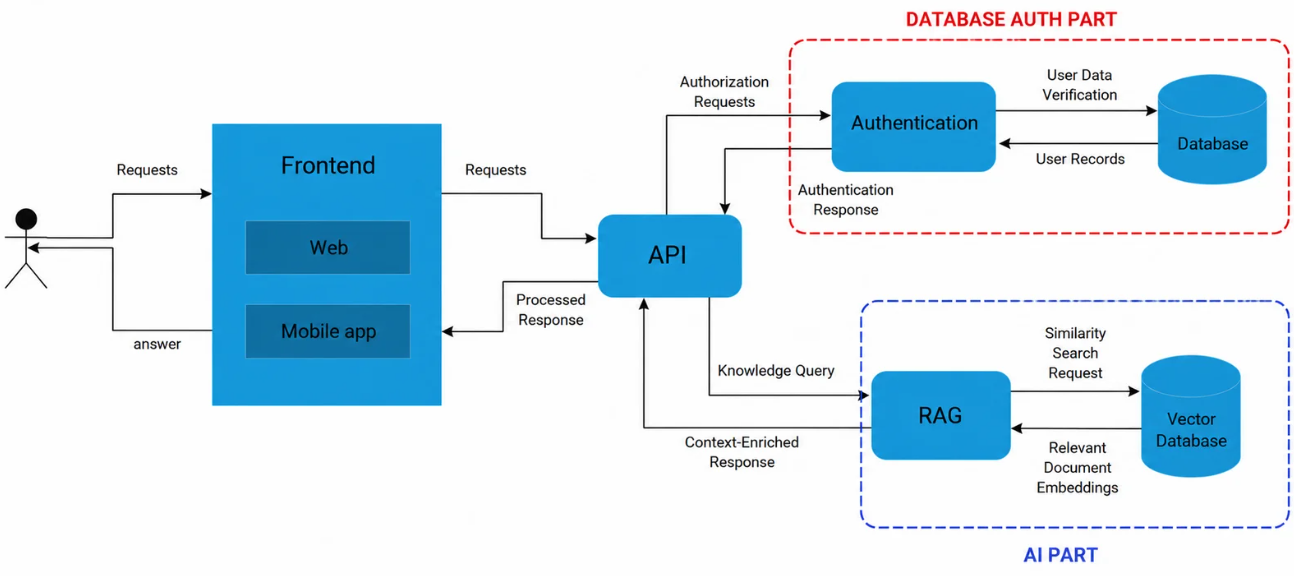
\includegraphics[width=0.82\textwidth]{system_block_diagram.png}
  }
  \caption{DocMind System Block Diagram.}
  \label{fig:block_diagram}
\end{figure}

\newpage

\subsection{Use Case Diagram}

Figure~\ref{fig:use_case} presents the use case diagram, which illustrates the interactions between system actors and core functionalities. It defines how students, instructors, and administrators interact with DocMind at a high level.

\begin{figure}[H]
  \centering
  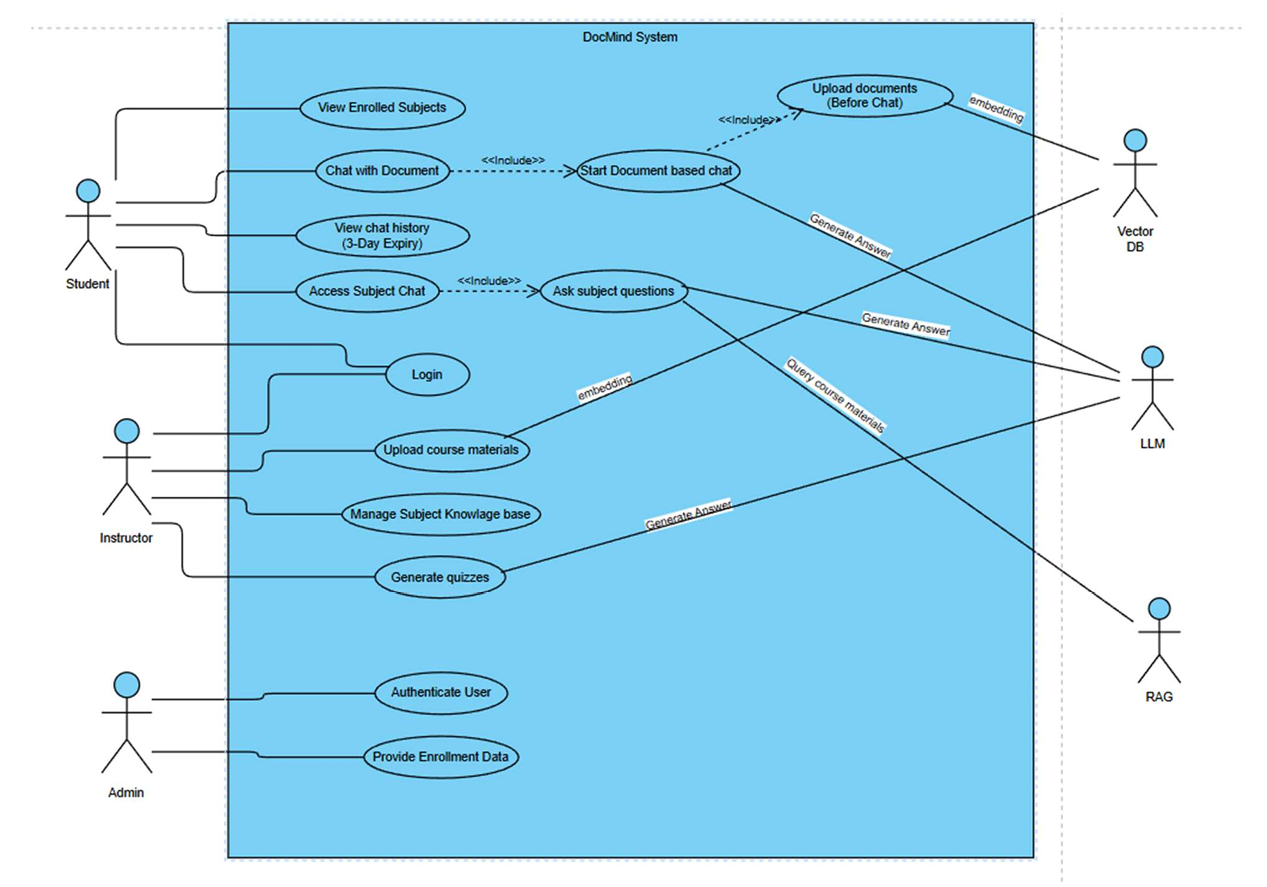
\includegraphics[width=1\textwidth]{use_case_diagram.png}
  \caption{DocMind Use Case Diagram.}
  \label{fig:use_case}
\end{figure}

\newpage

\subsection{Activity Diagram}

Figure~\ref{fig:activity} presents the activity diagram, which describes the flow of actions within the system, particularly for document-based chat interactions from the student's perspective. These diagrams clarify decision points, parallel actions, and system responses throughout the interaction process.

\begin{figure}[H]
  \centering
  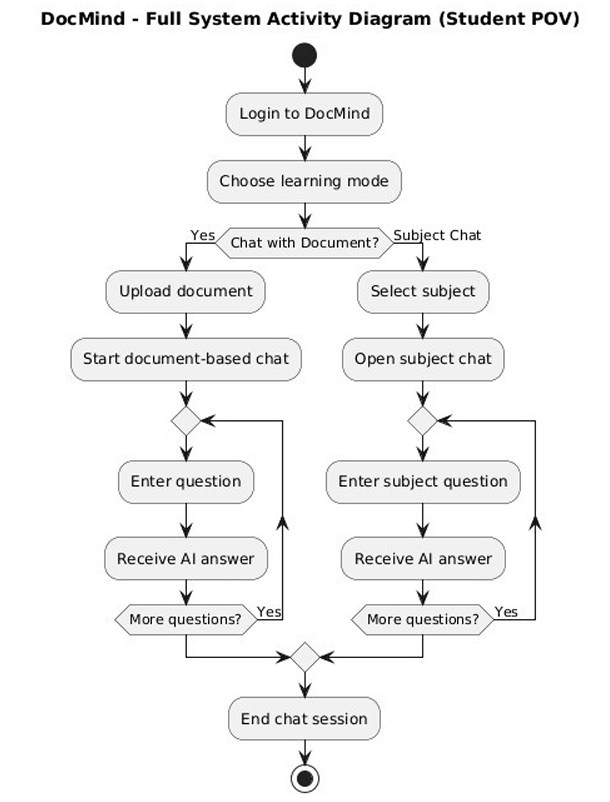
\includegraphics[width=0.75\textwidth]{activity_diagram.png}
  \caption{DocMind Full System Activity Diagram (Student POV).}
  \label{fig:activity}
\end{figure}

\subsection{Sequence Diagrams}

Sequence diagrams illustrate the time-ordered interaction between system components for the two primary chat flows.

\subsubsection{Document-Based Chat (RAG)}

Figure~\ref{fig:seq_rag} presents the sequence diagram for the document-based chat flow, showing how file upload and vector checking are orchestrated between the frontend, backend, and vector store.

\begin{figure}[H]
  \centering
  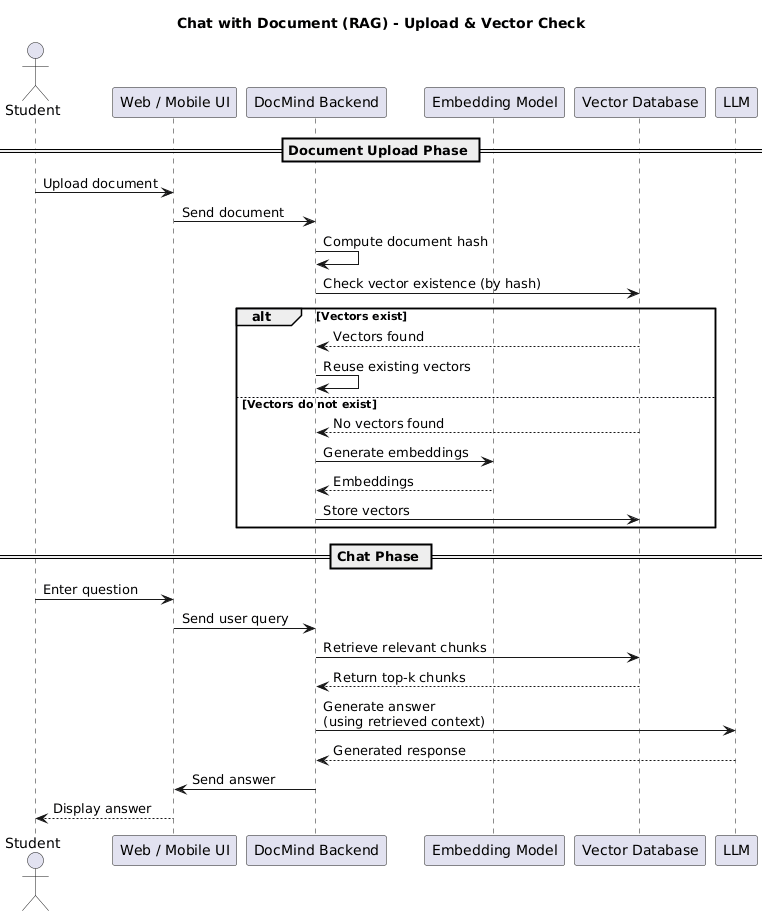
\includegraphics[width=0.8\textwidth]{sequence_diagram_rag.png}
  \caption{Chat with Document (RAG) -- Upload and Vector Check Sequence Diagram.}
  \label{fig:seq_rag}
\end{figure}

\newpage

\subsubsection{Subject-Based Chat}

Figure~\ref{fig:seq_subject} presents the sequence diagram for the subject-based chat flow, illustrating how instructor-uploaded materials are retrieved and used to ground the AI response.

\begin{figure}[H]
  \centering
  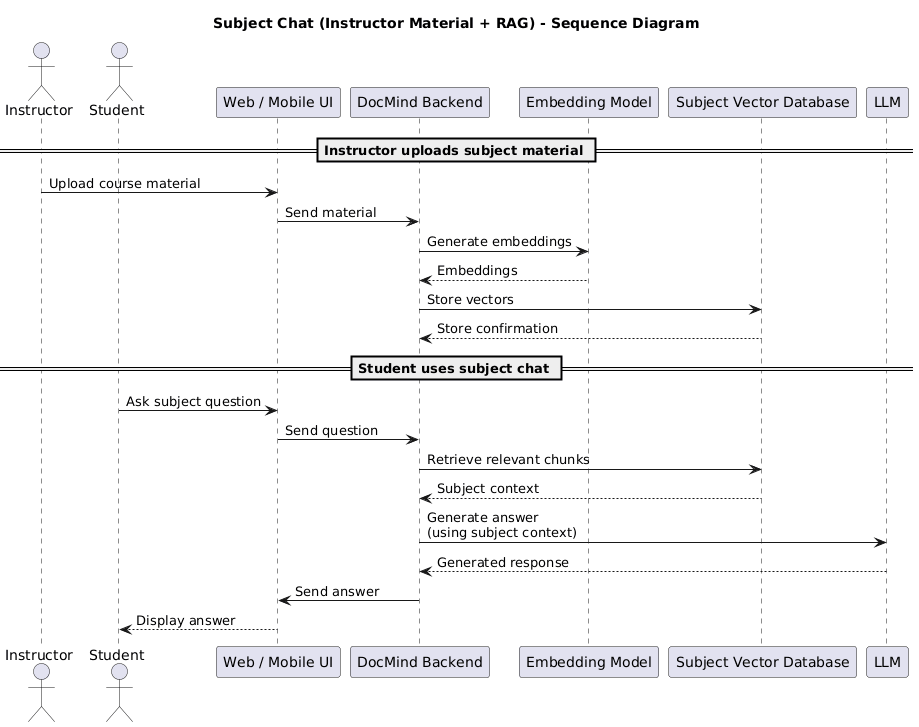
\includegraphics[width=0.9\textwidth]{sequence_diagram_subject.png}
  \caption{Subject Chat (Instructor Material and RAG) -- Sequence Diagram.}
  \label{fig:seq_subject}
\end{figure}

\newpage

\subsection{Database Design and ERD}

The database design is represented using an Entity-Relationship Diagram (ERD), which illustrates entities, attributes, and relationships. Figure~\ref{fig:erd} presents the full ERD for the DocMind system.

\begin{sidewaysfigure}
  \centering
  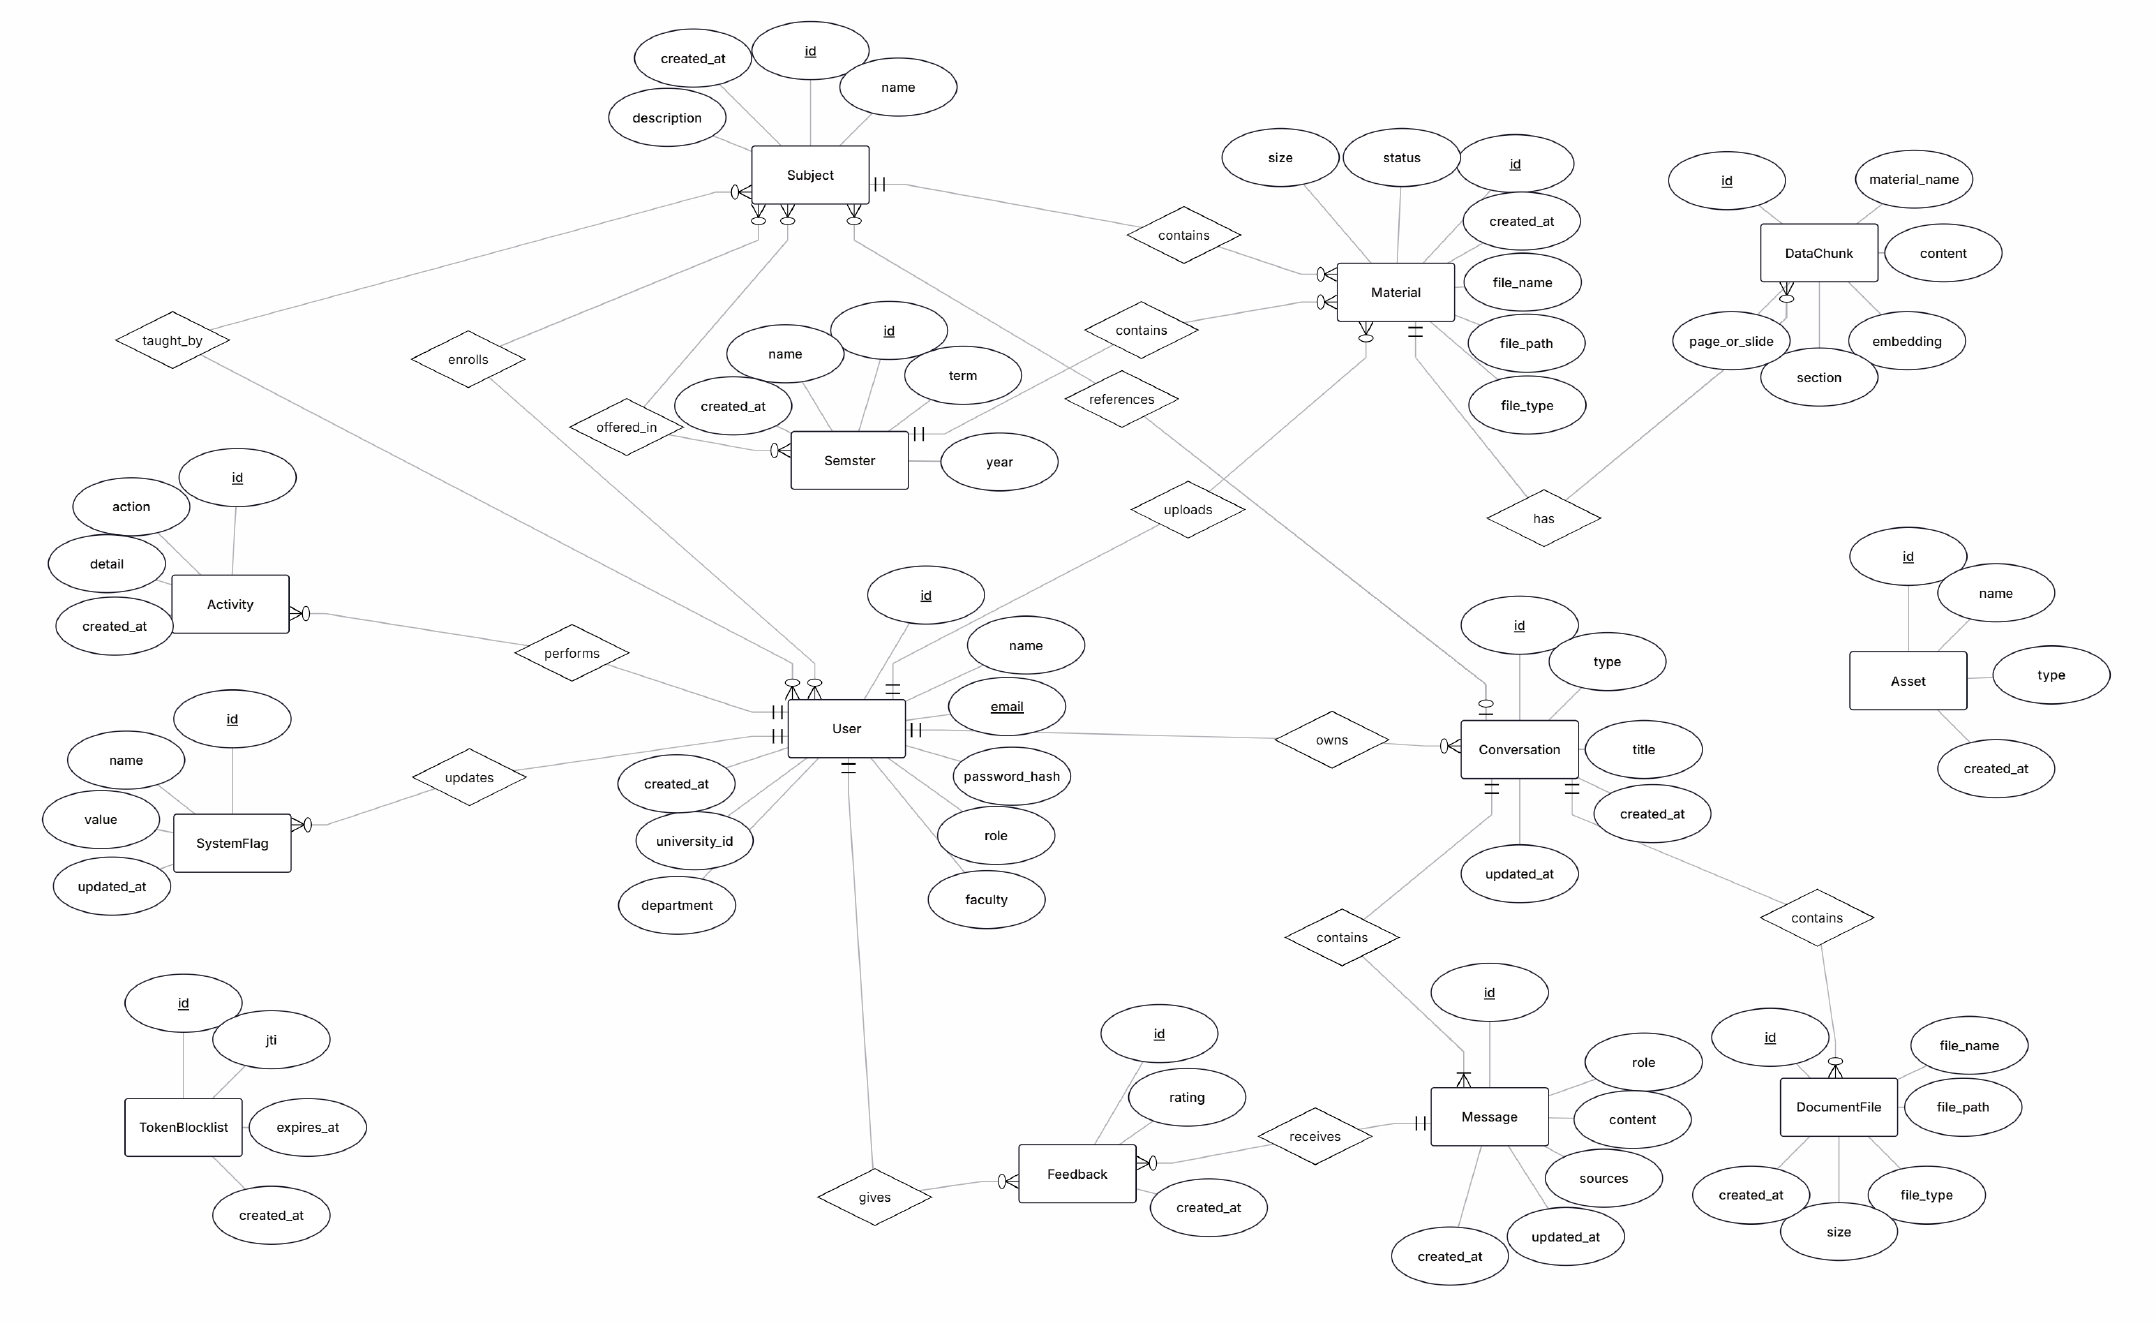
\includegraphics[width=\textheight]{erd.png}
  \caption{DocMind Entity-Relationship Diagram (ERD).}
  \label{fig:erd}
\end{sidewaysfigure}

\subsubsection{Entity-Level Design}

Each entity in the ERD shown in Figure~\ref{fig:erd} corresponds to a logical system component. Primary and foreign keys enforce relationships between users, subjects, documents, sessions, and embeddings. Subjects optionally reference a semester through a nullable foreign key that is cleared rather than cascaded when a semester is removed; each semester stores an optional start and end date from which its lifecycle state is derived in application code, so the state itself is not persisted.

\newpage

\subsection{Security Design}

Security is integrated into the system design at multiple levels. Authentication is handled within the application using password verification and JWT issuance; authorization is enforced through role-based access control on each route.

Production deployments are expected to use HTTPS end-to-end; passwords are stored hashed. Structured activity and admin endpoints support operational auditing; deeper anomaly detection would be added at the infrastructure layer.

\subsection{Error Handling and Fault Tolerance}

The system is designed to handle errors gracefully. Invalid inputs, expired sessions, unavailable services, and unexpected failures are managed through controlled error responses.

Fallback mechanisms and retries are implemented where appropriate to improve system robustness.

\subsection{Design Validation}

The design decisions described in this chapter are validated against the requirements defined in the previous sections. Each functional requirement is supported by one or more design components, ensuring full traceability.

This structured system design provides a solid foundation for implementation, testing, and future system enhancement.

% ════════════════════════════════════════════════════════════════════════════
%  CHAPTER 4 — IMPLEMENTATION AND TESTING
% ════════════════════════════════════════════════════════════════════════════
\chapter{Implementation and Testing}

This chapter describes the working implementation in the DocMind repository: a full-stack prototype comprising a FastAPI backend, PostgreSQL schema with Alembic migrations, optional pgvector or Qdrant for embeddings, and a React frontend. It demonstrates how the concepts, requirements, and design decisions from Chapter 3 are realized in code and in the running application.

The implementation covers the primary user journeys for students, instructors, and administrators, including authentication, document chat with file lifecycle and feedback, tutor (subject) chat over indexed materials, instructor material upload, and admin dashboards for users, subjects, analytics, feedback, activity, and student-access control.

\section{Technology Stack}

The DocMind system is implemented using the following technologies:

\begin{itemize}
  \item \textbf{Backend}: Python 3.10, FastAPI [12], SQLAlchemy (async), Alembic for migrations, Pydantic for data validation.
  \item \textbf{AI/ML}: an in-house Retrieval-Augmented Generation (RAG) orchestration layer (structure-aware chunking, prompt assembly, and retrieval) that uses LangChain text-splitting utilities [13]; embedding generation and text generation are served by configurable remote providers (OpenAI by default with ollama, Google Gemini, or Cohere), and an optional \texttt{sentence-transformers} cross-encoder is available for reranking.
  \item \textbf{Vector Store}: pgvector [15] (PostgreSQL extension) or Qdrant [16], switchable by environment configuration.
  \item \textbf{Relational Database}: PostgreSQL 16 with the pgvector extension.
  \item \textbf{Web Frontend}: React 19 with Vite, Tailwind CSS, React Router, and Axios for API calls.
  \item \textbf{Mobile}: Flutter and Dart, with GetX for state management and dependency injection and Dio for HTTP, organized in Clean Architecture (data, domain, and presentation layers per feature).
  \item \textbf{Authentication}: JSON Web Tokens (JWT), bcrypt password hashing, and token blocklist for logout.
  \item \textbf{Containerization}: Docker and Docker Compose for local development and deployment.
  \item \textbf{Version Control}: Git with GitHub, using a monorepo structure with separate backend, frontend, and mobile directories.
\end{itemize}

\newpage

\section{Backend Implementation}

\subsection{Project Structure}

The backend follows a layered architecture:

\begin{itemize}
  \item \textbf{Routers} (\texttt{/api/...}): Handle HTTP request routing and response serialization.
  \item \textbf{Services}: Contain business logic, orchestrate RAG operations, and enforce authorization constraints.
  \item \textbf{Repositories}: Abstract database access using SQLAlchemy async sessions.
  \item \textbf{Models}: Define SQLAlchemy ORM models and Pydantic schemas.
  \item \textbf{Core}: Configuration management (\texttt{settings.py}), security utilities, and dependency injection.
\end{itemize}

\subsection{Authentication and Authorization}

JSON Web Token (JWT)-based authentication is implemented in AuthService. On successful login, the service issues a signed access token embedding the user's identifier and role. Every protected route uses a FastAPI dependency that validates the token signature, checks expiry, and rejects token identifiers recorded in the blocklist. Role-specific dependencies (\texttt{require\_student}, \texttt{require\_instructor}, and \texttt{require\_admin}) are applied to route groups to enforce the principle of least privilege.

\newpage
\subsection{Document Ingestion Pipeline}

When a student uploads one or more PDF files to a document-based conversation, the backend performs the following steps:
\begin{enumerate}
  \item Validates the file type, MIME type, size, and per-conversation count against configured limits.
  \item Stores the file on disk and records metadata in the \texttt{documents} table.
  \item Triggers an asynchronous ingestion task that reads the PDF and splits it into structure-aware chunks: detected tables are emitted as atomic Markdown blocks, section headings (detected by relative font size) are prepended to each chunk as breadcrumbs, and prose is split recursively (paragraph, then line, then sentence) with a trailing-text overlap so that definitions and worked examples are not cut mid-thought. It then generates embeddings for each chunk and upserts the vectors into the conversation-scoped collection in the vector store.
  \item Updates the document's indexing status in the relational database so the frontend can display the current state (pending, indexed, or failed).
\end{enumerate}

\newpage

\subsection{RAG Query Pipeline}

When a student submits a message, the backend performs the following steps:
\begin{enumerate}
  \item The backend retrieves the top-$k$ most semantically similar chunks from the conversation or subject collection. When cross-encoder reranking is enabled (disabled by default), it over-fetches a larger candidate set by recall and a cross-encoder truncates it back to the top-$k$ by precision, soft-degrading to the original vector order on any fault.
  \item Each retrieved chunk carries its provenance (source filename, section heading, and page or slide); these are assembled into a context block, inserted into a prompt template available in English and Arabic locales, and the model is instructed to cite the sources it relied on. For subject chat, a short manifest of the subject's indexed materials is also supplied so the model knows what it can ground answers in.
  \item The prompt is sent to the configured LLM API (Gemini, OpenAI, or Cohere) for generation.
  \item The response is stored in the \texttt{messages} table, associated with the conversation, and returned to the client.
  \item Optionally, if the agentic mode is enabled, a planner model first decides whether retrieval is needed and with what reformulated query before the generator runs; it may additionally scope retrieval to specific instructor materials the student names (disabled by default).
\end{enumerate}

\subsection{Administrative APIs}

The admin router exposes endpoints for user Create, Read, Update, and Delete (CRUD) operations (create instructor accounts, activate or deactivate users, reset passwords), subject management, semester management (creating, updating, and deleting semesters with optional date windows, where subjects of a deleted semester are left unassigned rather than removed), aggregated statistics (daily message counts, subject-level activity, per-user usage), feedback records collected from student thumbs-up/down interactions, a global student-access flag that gates all student-facing routes with a configurable maintenance message, and a structured activity log recording every administrative action for audit review.

\newpage

\section{Frontend Implementation}

\subsection{Application Structure}

The React frontend is structured as a Single-Page Application (SPA) with protected routes guarded by the stored JWT. Navigation is organized around three role-specific views:

\begin{itemize}
  \item \textbf{Student}: Home dashboard, document-based chat, subject selection, and tutor chat.
  \item \textbf{Instructor}: Subject management dashboard with material upload, status tracking, and file management.
  \item \textbf{Administrator}: User management, subject management, semester management, analytics, feedback viewer, activity log, and system settings.
\end{itemize}

\subsection{State Management}

Application state is managed via React Context for authentication (token storage, decoded role, and logout trigger) and component-level state for chat history, upload progress, and indexing status. The frontend polls or listens for indexing status updates so that students receive real-time feedback during document processing.

\newpage

\section{Student Interface}

\subsection{Document-Based Chat Interface}

In document-based chat, students create a conversation with one or more PDF uploads within configured count and size limits. The backend saves files, runs ingestion and chunk embedding, and attaches vectors to a per-conversation collection. Students may add further PDF files to the same conversation up to the limit, then ask questions in a conversational interface while indexing states are shown in the User Interface (UI).

The chat interface displays user questions and system responses in a chronological format, allowing students to follow the conversation flow easily. Visual indicators are used to show system processing states, such as document indexing and response generation.

Figure~\ref{fig:student_doc} shows the student interface for document-based chat.

\begin{figure}[H]
  \centering
  \setlength{\fboxsep}{6pt}
  \setlength{\fboxrule}{0.8pt}
  \fbox{%
    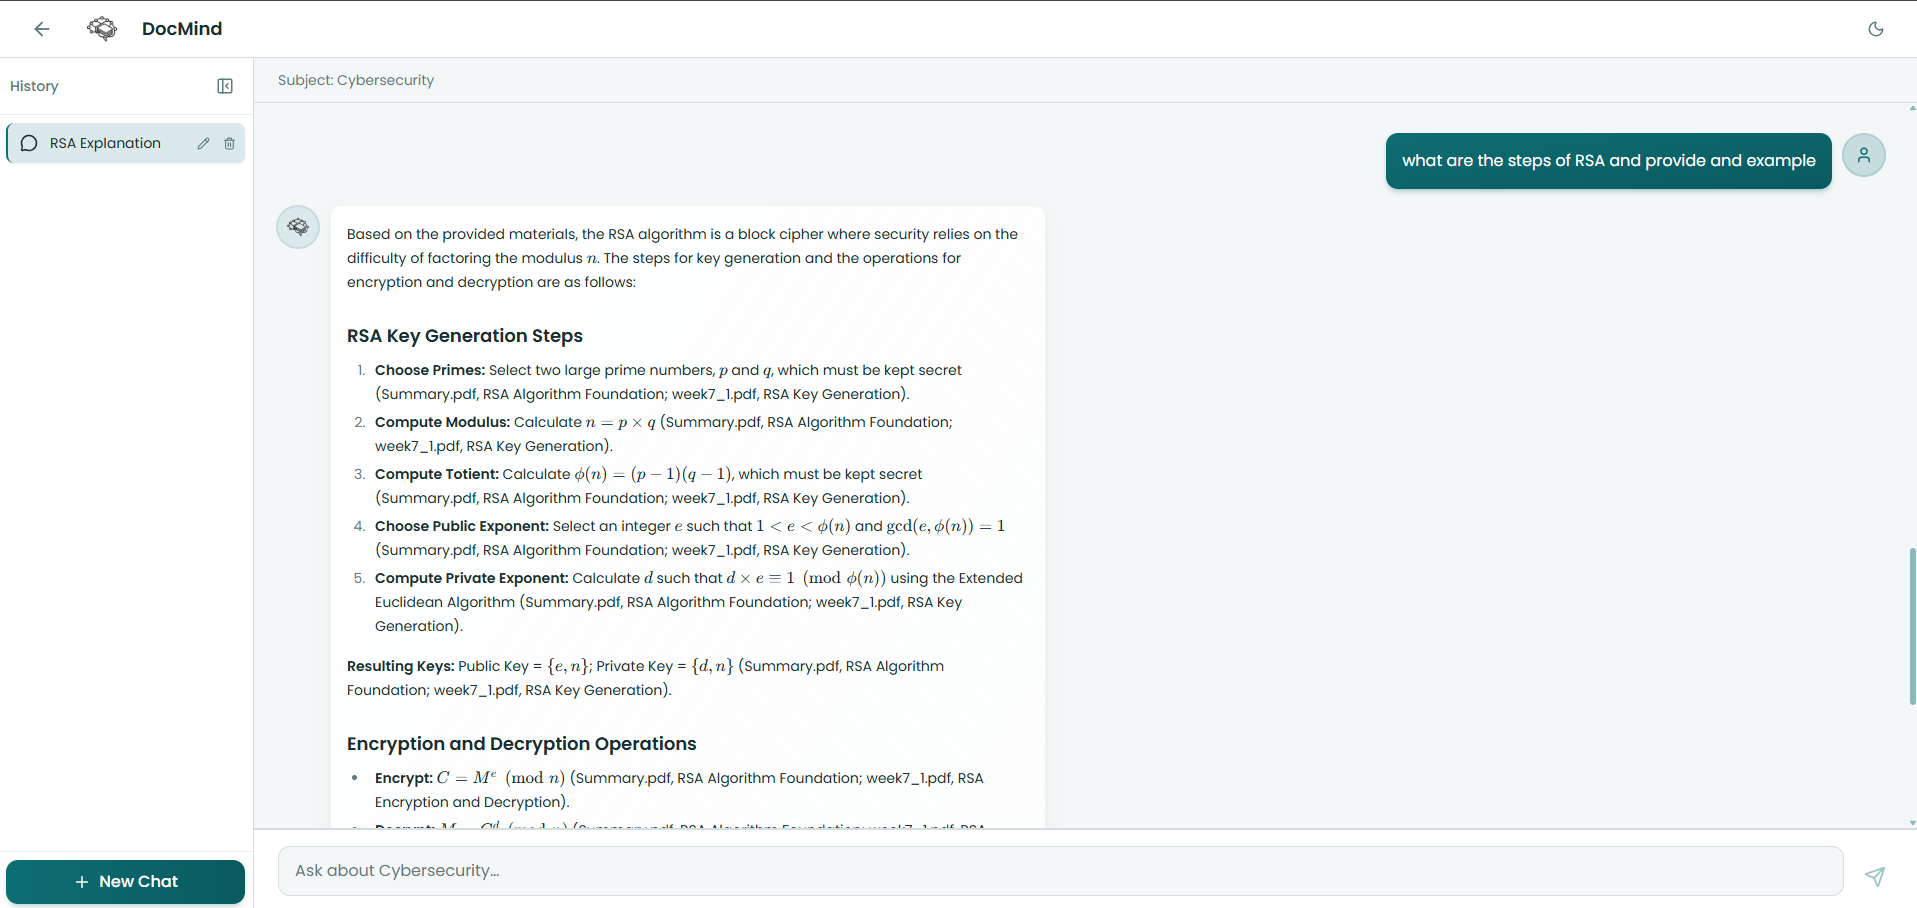
\includegraphics[width=0.82\textwidth]{prototype_student_docbased.png}
  }
  \caption{Student Interface -- Document-Based Chat.}
  \label{fig:student_doc}
\end{figure}

\newpage

\subsection{Subject-Based Chat Interface}

The tutor (subject-based) chat interface allows students to select a course or subject for which they are enrolled and for which instructors have uploaded materials. Subjects are presented with the most recent semester first, so the current term surfaces above older ones. Retrieval is limited to indexed content for that subject. The interface surfaces the active subject and instructor context so that answers remain visually tied to the chosen course. Subjects belonging to an archived semester are shown in a read-only state: their past conversations remain reviewable, but starting a new chat is disabled.

Figure~\ref{fig:student_subject} shows the student interface for subject-based chat.

\begin{figure}[H]
  \centering
  \setlength{\fboxsep}{6pt}
  \setlength{\fboxrule}{0.8pt}
  \fbox{%
    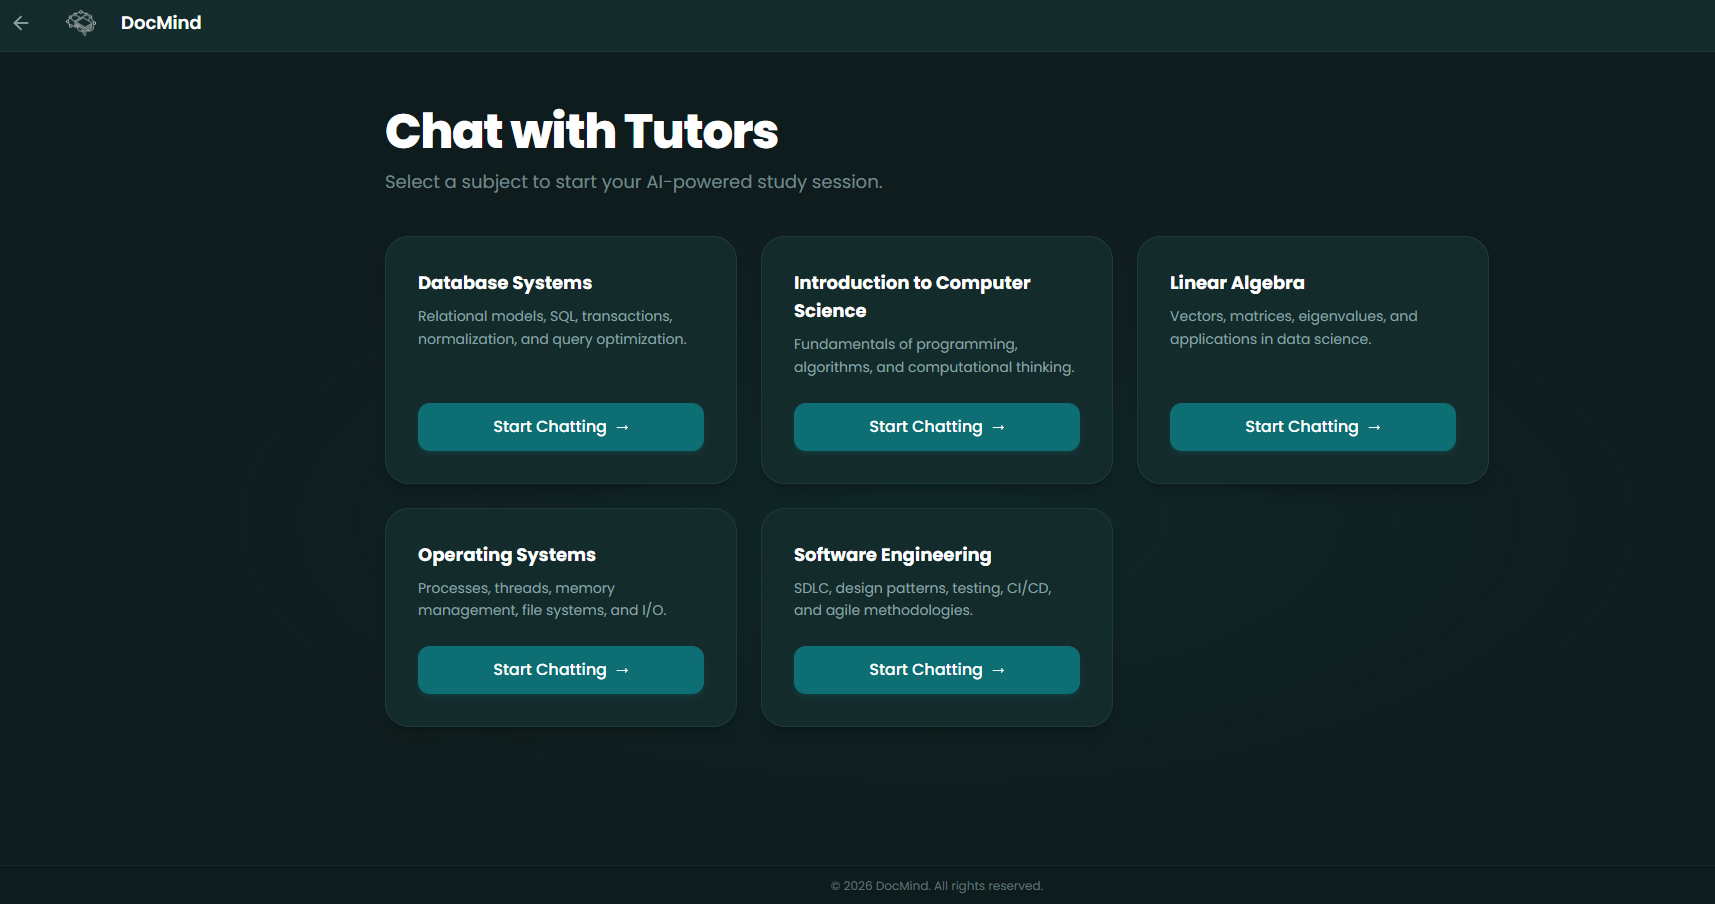
\includegraphics[width=0.82\textwidth]{prototype_student_subject.png}
  }
  \caption{Student Interface -- Subject-Based Chat (Chat with Tutors).}
  \label{fig:student_subject}
\end{figure}

\newpage

\section{Instructor Interface}

The instructor interface focuses on content management rather than acting as the chat tutor in the product flow. Instructors use a dashboard to open each assigned subject, upload or replace PDF materials, and observe processing status; aggregate analytics and cross-subject admin views are reserved for the administrator role in the current implementation.

\subsection{Content Management Interface}

Instructors can upload lecture notes, slides, and reference documents through a structured upload interface. The system automatically processes uploaded content and integrates it into the subject-specific knowledge base.

The interface provides feedback on upload status; the API rejects a new material when another material with the same display name already exists for that subject, which reduces accidental duplicate titles, though file-level byte deduplication is not implemented in the current codebase.

Figure~\ref{fig:instructor_content} shows the instructor content management dashboard.

\begin{figure}[H]
  \centering
  \setlength{\fboxsep}{6pt}
  \setlength{\fboxrule}{0.8pt}
  \fbox{%
    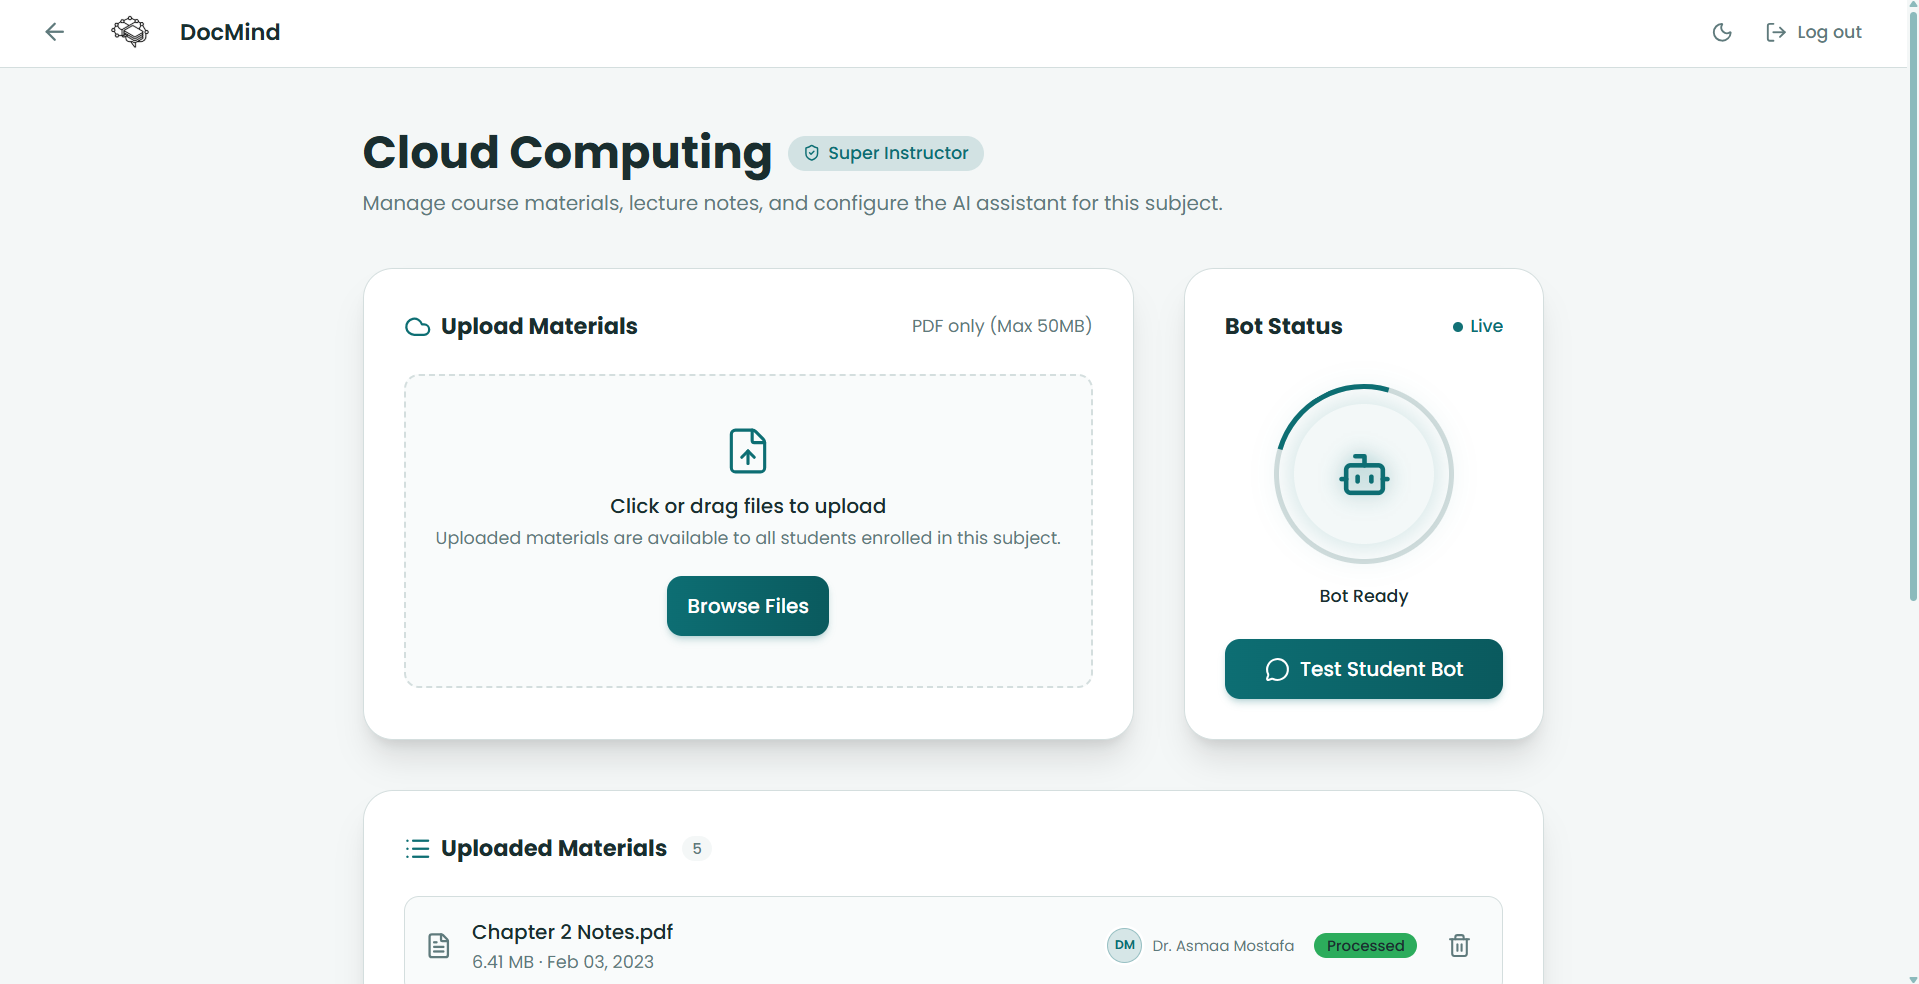
\includegraphics[width=0.82\textwidth]{prototype_instructor_content.png}
  }
  \caption{Instructor Interface -- Content Management Dashboard.}
  \label{fig:instructor_content}
\end{figure}

\newpage

\section{Testing}

\subsection{Testing Strategy}

The DocMind system employs a multi-level testing strategy to validate correctness, security, and usability:

\begin{itemize}
  \item \textbf{Unit Testing}: Individual service functions and repository methods are tested in isolation using pytest with async support. Mock objects are used to substitute external dependencies such as the vector store and LLM API.
  \item \textbf{Integration Testing}: API endpoints are tested end-to-end using an asynchronous HTTP client (\texttt{httpx.AsyncClient}) that drives the application in-process, exercising the full request-response cycle, including authentication, authorization, and database interaction, against a dedicated PostgreSQL with pgvector test database, while the language model and vector store are substituted with test doubles.
  \item \textbf{RAG Pipeline Testing}: The embedding and retrieval pipeline is validated by ingesting known documents and verifying that expected chunks are retrieved for representative queries.
  \item \textbf{Security Testing}: Role-Based Access Control (RBAC) is validated by asserting that requests made with student-role tokens are rejected by instructor and administrator endpoints, and vice versa.
  \item \textbf{User Acceptance Testing (UAT)}: Manual walkthroughs of the primary student, instructor, and administrator user journeys are performed against the running application with seeded data.
\end{itemize}

\subsection{Test Environment}

Testing is performed against a local Docker Compose environment that mirrors the production stack. Seeded users and subjects provide demo accounts and sample materials for repeatable test scenarios.

\newpage

\subsection{Test Cases}

Table~\ref{tab:test_cases} summarizes representative test cases executed during system validation.

\begin{table}[H]
\centering
\caption{Representative System Test Cases}
\label{tab:test_cases}
\begin{tabular}{>{\bfseries}p{1.5cm} p{4.5cm} p{4cm} p{3cm}}
\toprule
Test ID & Description & Expected Result & Status \\
\midrule
TC-01 & Student login with valid credentials & JWT issued, dashboard loaded & Pass \\
TC-02 & Student login with invalid password & 401 Unauthorized returned & Pass \\
TC-03 & Student accesses admin endpoint & 403 Forbidden returned & Pass \\
TC-04 & Upload valid PDF to document chat & File ingested, indexed, status shown & Pass \\
TC-05 & Upload invalid file type (DOCX) & 422 Unprocessable Entity returned & Pass \\
TC-06 & Ask question in document chat & RAG pipeline runs, answer returned & Pass \\
TC-07 & Ask question in subject chat & Subject-scoped retrieval, answer returned & Pass \\
TC-08 & Instructor uploads material with duplicate title & 409 Conflict returned & Pass \\
TC-09 & Admin disables student access & Students see maintenance message & Pass \\
TC-10 & Admin views analytics dashboard & Aggregated stats displayed correctly & Pass \\
TC-11 & Student submits thumbs-up feedback & Feedback stored, retrievable by admin & Pass \\
TC-12 & Logout and reuse token & 401 Unauthorized (token blocklisted) & Pass \\
TC-13 & Student starts tutor chat in an archived-semester subject & 403 Forbidden; past conversations remain readable & Pass \\
\bottomrule
\end{tabular}
\end{table}

\newpage

\subsection{Known Limitations and Remaining Gaps}

Remaining gaps are mainly operational and product-level rather than missing core flows. There is no native Single Sign-On (SSO) integration with a campus identity provider yet; encryption at rest and formal retention policies depend on hosting choices; rate limiting and horizontal autoscaling are not described in code as fixed guarantees; and automated test coverage is still growing.

Language models may still produce incorrect or out-of-context text despite RAG; the implementation mitigates this through retrieval, prompts, and optional agent routing, but does not eliminate model risk entirely.
\addtocontents{toc}{\protect\newpage}
\section{Prototype Evaluation}

Initial evaluation of the running system indicates that document-grounded and subject-grounded conversational learning paths function end-to-end with the stack described in this document. Beyond this functional confirmation, the answer quality of the Retrieval-Augmented Generation (RAG) pipeline was measured quantitatively using the RAGAS evaluation framework, as described in the following subsections. Stakeholder feedback and usage metrics, including optional per-message feedback stored for administrators, should inform further refinements to prompts, retrieval parameters, and User Experience (UX) design. This chapter documents the transition from system design to a concrete repository-backed implementation that can be demonstrated and extended toward production hardening.
\newpage
\subsection{Automated RAG Evaluation with RAGAS}

While the test cases in Table~\ref{tab:test_cases} confirm that each user journey behaves correctly, they do not measure how \emph{good} the generated answers are. To assess answer quality quantitatively, the RAG pipeline was evaluated with RAGAS, a reference-grounded, automated framework that uses a large language model as an independent judge to score retrieval-augmented answers along several complementary dimensions.

The evaluation harness reproduces the production pipeline so that the measured behavior matches the deployed system: the document ingestion and structure-aware chunking logic is ported verbatim from the backend ingestion service, the prompt templates are copied verbatim from the backend RAG templates, and retrieval mirrors the production search path. It was run over a curated question bank of 180 questions spanning 9 university subjects (communication skills, computer and society, computer graphics, computer system security, digital image processing, embedded systems, human-computer interaction, operating systems, and theory of computation), each paired with an instructor-style ground-truth answer. Retrieval parameters mirror the backend configuration (top-$k$ retrieval limit of 5 and a similarity threshold of 0.3), and generation and embedding are served by the configured local backend with ollama through OpenAI API, the \texttt{gemma4:e4b} generation model and the \texttt{qwen3-embedding:4b} embedding model, at a generation temperature of 0.2.

To quantify the benefit of the optional reranking stage, two retrieval configurations were scored head-to-head over the same question bank: a baseline that takes the top five vector-similarity matches (\textit{no-rerank}), and the optional cross-encoder path that over-fetches a larger candidate set and rescores it with a \texttt{BAAI/bge-reranker-base} cross-encoder before truncating back to the top five (\textit{with-rerank}). All answers were scored by RAGAS using an independent OpenAI judge model, so that answer quality is assessed by a different model than the one that produced the answers.

\newpage

\subsection{Evaluation Metrics}

Each answer was scored on five RAGAS metrics, all normalized to the range $[0, 1]$ where higher is better:

\begin{itemize}
  \item \textbf{Faithfulness}: the degree to which the claims in the answer are grounded in the retrieved context, directly measuring resistance to hallucination.
  \item \textbf{Answer Relevancy}: how directly and completely the answer addresses the question that was asked.
  \item \textbf{Context Precision}: the proportion of retrieved chunks that are actually relevant to the question, reflecting retrieval quality.
  \item \textbf{Context Recall}: whether the retrieved context covers the information present in the ground-truth answer.
  \item \textbf{Answer Correctness}: the overall agreement between the generated answer and the ground-truth answer.
\end{itemize}

\subsection{Evaluation Results}

Table~\ref{tab:ragas_summary} reports the mean score for each metric across all 180 questions for both retrieval configurations, and Table~\ref{tab:ragas_subjects} breaks the overall score down by subject.

\begin{table}[H]
\centering
\caption{Mean RAGAS Scores Across 180 Questions (No-Rerank vs.\ With-Rerank)}
\label{tab:ragas_summary}
\begin{tabular}{>{\bfseries}p{5cm} c c}
\toprule
Metric & No-Rerank & With-Rerank \\
\midrule
Faithfulness        & 0.942 & 0.959 \\
Answer Relevancy    & 0.777 & 0.786 \\
Context Precision   & 0.908 & 0.926 \\
Context Recall      & 0.915 & 0.914 \\
Answer Correctness  & 0.768 & 0.776 \\
\midrule
\textbf{Mean (5 metrics)} & \textbf{0.862} & \textbf{0.872} \\
\bottomrule
\end{tabular}
\end{table}

\begin{table}[H]
\centering
\caption{Mean RAGAS Score per Subject (Averaged Across the Five Metrics)}
\label{tab:ragas_subjects}
\begin{tabular}{>{\bfseries}p{6cm} c c c}
\toprule
Subject & No-Rerank & With-Rerank & Delta \\
\midrule
Communication Skills       & 0.891 & 0.902 & $+0.011$ \\
Computer and Society       & 0.864 & 0.922 & $+0.058$ \\
Computer Graphics          & 0.854 & 0.853 & $-0.001$ \\
Computer System Security   & 0.927 & 0.919 & $-0.008$ \\
Digital Image Processing   & 0.761 & 0.740 & $-0.021$ \\
Embedded Systems           & 0.837 & 0.845 & $+0.008$ \\
Human-Computer Interaction & 0.924 & 0.928 & $+0.004$ \\
Operating Systems          & 0.882 & 0.889 & $+0.007$ \\
Theory of Computation      & 0.817 & 0.850 & $+0.033$ \\
\bottomrule
\end{tabular}
\end{table}

The results validate the core design premise of DocMind. High faithfulness (approximately 0.94--0.96) together with strong context precision and recall (approximately 0.91--0.93) confirm that the pipeline retrieves the right material and that generated answers remain anchored to it rather than to model priors, the central mechanism by which RAG curbs hallucination in an academic setting. The comparatively lower answer relevancy and answer correctness scores (approximately 0.77) reflect differences in phrasing and completeness relative to the strict instructor-authored ground truth rather than failures of grounding, an outcome consistent with the use of a compact, locally hosted generation model.

Enabling cross-encoder reranking produces a small but consistent improvement in the overall mean score (from 0.862 to 0.872), with the clearest gains in faithfulness and context precision. The per-subject breakdown in Table~\ref{tab:ragas_subjects} shows that this benefit is uneven: reranking helps markedly on subjects such as Computer and Society and Theory of Computation, while leaving others essentially unchanged or marginally lower (for example, Digital Image Processing). This mixed, modest effect at additional latency and dependency cost is precisely why reranking ships as an optional, off-by-default stage in the RAG query pipeline, and why hybrid and query-expansion retrieval are identified as future enhancements.

% ════════════════════════════════════════════════════════════════════════════
%  CHAPTER 5 — CONCLUSIONS AND FUTURE WORK
% ════════════════════════════════════════════════════════════════════════════
\chapter{Conclusions and Future Work}

\section{Conclusions}

The DocMind project successfully demonstrates the feasibility of integrating a trustworthy, document-grounded AI assistant into a university academic environment. By employing Retrieval-Augmented Generation (RAG) over explicitly managed document corpora, the system substantially reduces the risk of hallucination compared to unrestricted language model deployments, ensuring that student responses remain anchored to verified course materials.

The implemented system achieves all primary objectives set out in Chapter 1. Role-Based Access Control (RBAC) effectively separates student, instructor, and administrator concerns. The dual interaction model, encompassing both document-based chat and subject-based tutor chat, addresses different student learning scenarios within a unified interface. JSON Web Token (JWT)-based authentication with configurable token lifetime and a blocklist-based logout mechanism provides session security appropriate for institutional deployment.

The literature review confirmed that plain RAG, without necessarily fine-tuning the underlying model, is a practical and cost-effective strategy for domain-specific question-and-answer applications [5]. Paper findings from Barnett et al.\ [3] reinforced this by demonstrating that fine-tuning may degrade RAG performance in specialized domains, while Li et al.\ [4] showed that prompt engineering and retrieval quality have greater impact on answer accuracy than knowledge base size. These insights directly shaped the DocMind retrieval pipeline design.

The market survey revealed that while commercial tools such as NotebookLM [17], Humata [18], Mindgrasp [19], and AskYourPDF [20] offer overlapping document-chat features, none are designed for institutional multi-role deployment with instructor-controlled knowledge bases. DocMind fills this gap by providing an open, configurable system that institutions can deploy and operate without per-user subscription costs.

\newpage

In conclusion, DocMind demonstrates that it is possible to build an academically responsible AI assistant that is reliable, role-aware, and deployable within university infrastructure using accessible open-source technologies. The system represents a meaningful contribution to the intersection of artificial intelligence and higher education, providing a foundation that can be extended, hardened for production, and adopted by institutions seeking to improve student learning outcomes without compromising academic integrity.

\section{Future Work}

While the current implementation realizes the core functionality of DocMind, several enhancements are planned to increase the system's robustness, reach, and academic utility. The following subsections describe the most significant planned directions.

\subsection{Single Sign-On Integration}

The current authentication model uses application-managed credentials. Future work will extend the authentication layer to support Security Assertion Markup Language (SAML) 2.0 or OAuth 2.0 federation with institutional identity providers (such as Lightweight Directory Access Protocol (LDAP), Active Directory, or university Single Sign-On (SSO) portals), eliminating the need for separate account provisioning and aligning with institutional security policies.

\subsection{Multi-Language Support}

Although the system includes English and Arabic prompt templates, the user interface is primarily English. Future versions will provide a fully localized Arabic interface and extend the language model prompt templates to support additional languages relevant to the institution's student population.

\subsection{Automated Quiz and Assessment Generation}

A natural extension of the subject-based chat is the ability for instructors to trigger AI-generated quiz questions from uploaded materials. These would be reviewed and published by the instructor before being made available to students, maintaining instructor control while automating a time-consuming task.
\newpage
\subsection{Enhanced Retrieval Strategies}

The RAG pipeline already supports optional cross-encoder reranking to improve the precision of the top-$k$ retrieved chunks, and optional source-scoped retrieval that restricts a query to specific instructor materials; both are disabled by default and can be enabled per deployment. Future improvements, informed by best-practice findings in [4], include hybrid retrieval combining dense vector search with keyword-based (BM25) sparse retrieval, and query expansion using lightweight models to improve recall for short or ambiguous student queries.

\subsection{Analytics and Learning Insights}

The administrator analytics dashboard currently provides usage-level metrics. Future work will introduce learning-oriented analytics, such as frequently asked concept clusters per subject, knowledge gap detection based on question patterns, and per-student engagement trends. These insights would assist instructors in adapting their course materials to student needs.

\subsection{Production Hardening}

Operational improvements include formal rate limiting on all API endpoints to prevent abuse, encryption at rest for the relational database and vector store, automated integration and regression test coverage tracking, horizontal autoscaling configuration for cloud deployments using Kubernetes-based orchestration, and formal data retention and deletion policies compliant with the General Data Protection Regulation (GDPR) [11] and institutional data governance frameworks.

\subsection{Agentic Retrieval Expansion}

The optional agentic layer (plan-execute-reflect) is disabled by default in the current implementation. Future work will mature this component, evaluate its impact on answer quality and latency, and promote it as the default retrieval strategy once stability is confirmed.

% ════════════════════════════════════════════════════════════════════════════
%  REFERENCES
% ════════════════════════════════════════════════════════════════════════════
\chapter*{References}
\addcontentsline{toc}{chapter}{References}

\begin{list}{[\arabic{enumi}]}{\usecounter{enumi}\setlength{\leftmargin}{2.5em}\setlength{\itemsep}{6pt}}

  \item H.\ Zamani and A.\ Salemi, ``Comparing Retrieval-Augmentation and Parameter Efficient Fine-Tuning for Privacy-Preserving Personalization of Large Language Models,'' University of Massachusetts, Jun.\ 2025.

  \item N.\ Lawton, A.\ Samuel, A.\ Kumar, and D.\ Liu, ``A Comparison of Independent and Joint Fine-Tuning Strategies for Retrieval-Augmented Generation,'' Cornell University, Oct.\ 2025.

  \item S.\ Barnett, Z.\ Brannelly, Stefanus, and S.\ Wong, ``Fine-Tuning or Fine-Failing? Debunking Performance Myths in Large Language Models,'' Deakin University, Jun.\ 2025.

  \item S.\ Li, L.\ Stenzel, C.\ Eickhoff, and S.\ Ali, ``Enhancing Retrieval-Augmented Generation: A Study of Best Practices,'' University of T\"{u}bingen, Jan.\ 2025.

  \item P.\ Lewis, E.\ Perez, A.\ Piktus, et al., ``Retrieval-Augmented Generation for Knowledge-Intensive NLP Tasks,'' in \textit{Advances in Neural Information Processing Systems (NeurIPS)}, 2020.

  \item W.\ Holmes, M.\ Bialik, and C.\ Fadel, \textit{Artificial Intelligence in Education: Promises and Implications for Teaching and Learning}. Boston, MA: Center for Curriculum Redesign, 2019.

  \item D.\ Jurafsky and J.\ H.\ Martin, \textit{Speech and Language Processing}, 3rd ed. Upper Saddle River, NJ: Pearson, 2023.

  \item I.\ Sommerville, \textit{Software Engineering}, 10th ed. Harlow, UK: Pearson, 2016.

  \item ISO/IEC/IEEE 29148:2018, \textit{Systems and Software Engineering Life Cycle Processes Requirements Engineering}, IEEE Standards Association, 2018.

  \item OWASP Foundation, \textit{OWASP Top Ten Web Application Security Risks}, 2023. [Online]. Available: \url{https://owasp.org/www-project-top-ten/} (Last access Oct.\ 2025).

  \item European Union, ``General Data Protection Regulation (GDPR),'' Regulation (EU) 2016/679, Off.\ J.\ Eur.\ Union, Apr.\ 2016.

  \item S.\ Tiangolo, \textit{FastAPI: Modern, Fast Web Framework for Building APIs with Python}. [Online]. Available: \url{https://fastapi.tiangolo.com} (Last access Oct.\ 2025).

  \item J.\ Harrison, \textit{LangChain: Building Applications with LLMs}. [Online]. Available: \url{https://python.langchain.com} (Last access Oct.\ 2025).

  \item A.\ Johnson et al., ``FAISS: A Library for Efficient Similarity Search,'' Facebook AI Research. [Online]. Available: \url{https://github.com/facebookresearch/faiss} (Last access Oct.\ 2025).

  \item pgvector Contributors, \textit{pgvector: Open-Source Vector Similarity Search for PostgreSQL}. [Online]. Available: \url{https://github.com/pgvector/pgvector} (Last access Mar.\ 2026).

  \item Qdrant Team, \textit{Qdrant Vector Database Documentation}. [Online]. Available: \url{https://qdrant.tech/documentation/} (Last access Oct.\ 2025).

  \item Google, \textit{NotebookLM: AI-Powered Research and Learning Tool}. [Online]. Available: \url{https://notebooklm.google.com} (Last access Oct.\ 2025).

  \item Humata AI, \textit{Humata: AI-Powered Document Assistant}. [Online]. Available: \url{https://www.humata.ai} (Last access Oct.\ 2025).

  \item Mindgrasp, \textit{Mindgrasp: AI Learning and Study Platform}. [Online]. Available: \url{https://mindgrasp.ai} (Last access Oct.\ 2025).

  \item AskYourPDF, \textit{AskYourPDF: Chat with Your Documents}. [Online]. Available: \url{https://askyourpdf.com} (Last access Oct.\ 2025).

\end{list}

\end{document}